% Options for packages loaded elsewhere
\PassOptionsToPackage{unicode}{hyperref}
\PassOptionsToPackage{hyphens}{url}
\PassOptionsToPackage{dvipsnames,svgnames,x11names}{xcolor}
%
\documentclass[
  number,
  preprint,
  3p,
  onecolumn]{elsarticle}

\usepackage{amsmath,amssymb}
\usepackage{iftex}
\ifPDFTeX
  \usepackage[T1]{fontenc}
  \usepackage[utf8]{inputenc}
  \usepackage{textcomp} % provide euro and other symbols
\else % if luatex or xetex
  \usepackage{unicode-math}
  \defaultfontfeatures{Scale=MatchLowercase}
  \defaultfontfeatures[\rmfamily]{Ligatures=TeX,Scale=1}
\fi
\usepackage{lmodern}
\ifPDFTeX\else  
    % xetex/luatex font selection
\fi
% Use upquote if available, for straight quotes in verbatim environments
\IfFileExists{upquote.sty}{\usepackage{upquote}}{}
\IfFileExists{microtype.sty}{% use microtype if available
  \usepackage[]{microtype}
  \UseMicrotypeSet[protrusion]{basicmath} % disable protrusion for tt fonts
}{}
\makeatletter
\@ifundefined{KOMAClassName}{% if non-KOMA class
  \IfFileExists{parskip.sty}{%
    \usepackage{parskip}
  }{% else
    \setlength{\parindent}{0pt}
    \setlength{\parskip}{6pt plus 2pt minus 1pt}}
}{% if KOMA class
  \KOMAoptions{parskip=half}}
\makeatother
\usepackage{xcolor}
\setlength{\emergencystretch}{3em} % prevent overfull lines
\setcounter{secnumdepth}{5}
% Make \paragraph and \subparagraph free-standing
\ifx\paragraph\undefined\else
  \let\oldparagraph\paragraph
  \renewcommand{\paragraph}[1]{\oldparagraph{#1}\mbox{}}
\fi
\ifx\subparagraph\undefined\else
  \let\oldsubparagraph\subparagraph
  \renewcommand{\subparagraph}[1]{\oldsubparagraph{#1}\mbox{}}
\fi


\providecommand{\tightlist}{%
  \setlength{\itemsep}{0pt}\setlength{\parskip}{0pt}}\usepackage{longtable,booktabs,array}
\usepackage{calc} % for calculating minipage widths
% Correct order of tables after \paragraph or \subparagraph
\usepackage{etoolbox}
\makeatletter
\patchcmd\longtable{\par}{\if@noskipsec\mbox{}\fi\par}{}{}
\makeatother
% Allow footnotes in longtable head/foot
\IfFileExists{footnotehyper.sty}{\usepackage{footnotehyper}}{\usepackage{footnote}}
\makesavenoteenv{longtable}
\usepackage{graphicx}
\makeatletter
\def\maxwidth{\ifdim\Gin@nat@width>\linewidth\linewidth\else\Gin@nat@width\fi}
\def\maxheight{\ifdim\Gin@nat@height>\textheight\textheight\else\Gin@nat@height\fi}
\makeatother
% Scale images if necessary, so that they will not overflow the page
% margins by default, and it is still possible to overwrite the defaults
% using explicit options in \includegraphics[width, height, ...]{}
\setkeys{Gin}{width=\maxwidth,height=\maxheight,keepaspectratio}
% Set default figure placement to htbp
\makeatletter
\def\fps@figure{htbp}
\makeatother

\usepackage{booktabs}
\usepackage{caption}
\usepackage{longtable}
\usepackage{colortbl}
\usepackage{array}
\usepackage{dcolumn}
\usepackage{typearea}
\makeatletter
\@ifpackageloaded{caption}{}{\usepackage{caption}}
\AtBeginDocument{%
\ifdefined\contentsname
  \renewcommand*\contentsname{Table of contents}
\else
  \newcommand\contentsname{Table of contents}
\fi
\ifdefined\listfigurename
  \renewcommand*\listfigurename{List of Figures}
\else
  \newcommand\listfigurename{List of Figures}
\fi
\ifdefined\listtablename
  \renewcommand*\listtablename{List of Tables}
\else
  \newcommand\listtablename{List of Tables}
\fi
\ifdefined\figurename
  \renewcommand*\figurename{Figure}
\else
  \newcommand\figurename{Figure}
\fi
\ifdefined\tablename
  \renewcommand*\tablename{Table}
\else
  \newcommand\tablename{Table}
\fi
}
\@ifpackageloaded{float}{}{\usepackage{float}}
\floatstyle{ruled}
\@ifundefined{c@chapter}{\newfloat{codelisting}{h}{lop}}{\newfloat{codelisting}{h}{lop}[chapter]}
\floatname{codelisting}{Listing}
\newcommand*\listoflistings{\listof{codelisting}{List of Listings}}
\makeatother
\makeatletter
\makeatother
\makeatletter
\@ifpackageloaded{caption}{}{\usepackage{caption}}
\@ifpackageloaded{subcaption}{}{\usepackage{subcaption}}
\makeatother
\ifLuaTeX
  \usepackage{selnolig}  % disable illegal ligatures
\fi
\usepackage[]{natbib}
\bibliographystyle{elsarticle-num}
\usepackage{bookmark}

\IfFileExists{xurl.sty}{\usepackage{xurl}}{} % add URL line breaks if available
\urlstyle{same} % disable monospaced font for URLs
\hypersetup{
  pdftitle={Unveiling Adaptive Pedagogy: Reinforcement Learning Models Illuminate Teacher Decision-Making in an Online Math-Teaching Platform},
  pdfauthor={Marcos Gallo},
  pdfkeywords={Reinforcement Learning, Pedagogical Decision-Making,
Digital Education Platforms, Instructional Adaptation, Q-learning,
Actor-Critic},
  colorlinks=true,
  linkcolor={blue},
  filecolor={Maroon},
  citecolor={Blue},
  urlcolor={Blue},
  pdfcreator={LaTeX via pandoc}}

\setlength{\parindent}{6pt}
\begin{document}

\begin{frontmatter}
\title{Unveiling Adaptive Pedagogy: Reinforcement Learning Models
Illuminate Teacher Decision-Making in an Online Math-Teaching Platform}
\author[]{Marcos Gallo%
%
}



\cortext[cor1]{Corresponding author}

        
\begin{abstract}
This study introduces a new use of reinforcement learning (RL) models to
gain insight into teachers' decision-making processes on the Zearn
online math-teaching platform. Analyzing data from 3029 classrooms, our
approach treats pedagogical decision-making as a complex adaptive
system, taking into account educators' reward history and the unique
contexts of their instructional environments. Using Q-learning and
Actor-Critic models, we identify distinct patterns of teaching behavior.
Our comparison of RL models with a traditional logistic regression
baseline demonstrates the superiority of the Actor-Critic model in
capturing teacher behavior across most classrooms. Importantly, our
findings reveal a strong positive correlation between the learning rates
of state value weights and improved student achievement within the
preferred Actor-Critic model. This finding highlights educators'
adaptability in meeting their students' evolving needs in the digital
learning landscape, ultimately leading to better learning outcomes. By
demonstrating the relevance of RL models in the educational domain, our
study introduces a new approach to exploring teacher decision-making and
showcases their potential to inform the development of more effective,
adaptive teaching strategies.
\end{abstract}





\begin{keyword}
    Reinforcement Learning, Pedagogical Decision-Making, Digital
Education Platforms, Instructional Adaptation, Q-learning,
Actor-Critic \sep 
    Reinforcement Learning, Pedagogical Decision-Making, Digital
Education Platforms, Instructional Adaptation, Q-learning, Actor-Critic
\end{keyword}
\end{frontmatter}
    
\section{Introduction}\label{introduction}

Predicting repeated behavior has been a long-standing goal of the
behavioral sciences, including economics, psychology, and neuroscience.
Much of human behavior results from stimulus-response associations,
which are context-sensitive and not always consciously deliberated
\citep{buyalskaya2023}. Reinforcement learning (RL) algorithms have
emerged as a prominent way of quantifying these relationships, assigning
a mathematical relationship between contextual cues (states), behavior
(actions), and reward \citep{sutton2018}. These algorithms have found
wide application in neuroscience and cognitive psychology, where they
are used on data sets to model agents in specific environments. However,
these disciplines generally do not work with the practical and applied
data typically used in social psychology and economics
\citep{buyalskaya2023}.

This gap presents a novel opportunity to use methods from one set of
disciplines on data traditionally used in another. In this paper, we aim
to further this integration by applying RL algorithms to model the
decision-making process of teachers in the math-teaching platform Zearn.
Reinforcement learning (RL) provides a system of rewards and punishments
where the agent (in this case, the teacher) learns to make optimal
decisions by maximizing the rewards and minimizing the punishments. By
assuming every teacher has an objective function to balance with their
potential rewards, we model the sequential behavior of a teacher
throughout a school year. For instance, the teacher chooses which
pedagogical actions to employ, such as assigning homework, checking
student progress, or reviewing content, in anticipation of enhancing
student achievement. Applying RL algorithms allows for flexibility in
learning the best strategy given certain contextual information,
revealing the intricate dynamics of the teaching-learning process. That
is, we provide a model of how teachers adapt their strategies in
response to student performance and other contextual factors. This
approach offers a flexible and robust model for our available data and
opens new avenues for understanding and enhancing human behavior in
field settings.

\subsection{The Zearn Platform}\label{the-zearn-platform}

Zearn is a digital platform for mathematics education designed to
facilitate the teaching and learning of mathematics. About 25\% of
elementary school students and over 1 million middle school students
across the United States use Zearn \citep{post-weblog}. Its unique blend
of hands-on teaching and immersive digital learning, paired with its
widespread adoption, provides the perfect setting for understanding how
teachers adapt their strategies to optimize student achievement.

Zearn's pedagogical approach includes interactive digital lessons using
visual aids (see Figure~\ref{fig-zearn-poster}) and real-time student
feedback. The platform's approach to mathematical concepts, such as
fractions, is particularly noteworthy. Students go through a series of
representations: concrete, pictorial, and abstract, each designed to
scaffold their understanding (i.e., ``breaking down'' problems, see
\citep{jumaat2014, reiser2014}) and prepare them for subsequent levels.

\begin{figure}

\centering{

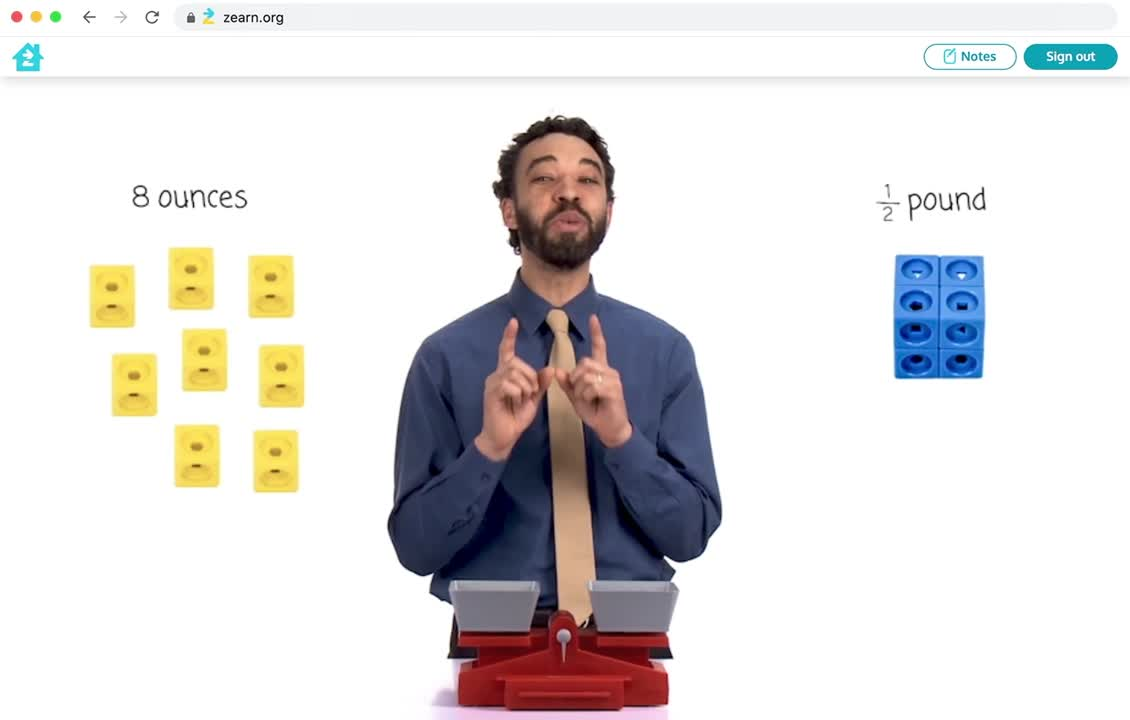
\includegraphics{images/zearn-poster.jpg}

}

\caption{\label{fig-zearn-poster}Example of Teaching with Visual Models
on Zearn}

\end{figure}%

The platform's structure facilitates a personalized learning experience
for students (see SI for a screenshot of the student portal), allowing
teachers to track student progress and make informed decisions (see
Figure~\ref{fig-class-report} for a sample class report). This structure
includes self-paced online lessons and small group instruction, a
rotational model that allows students to learn new grade-level content
in two ways: independently through engaging digital lessons and in small
groups with their teacher and classmates. This dual approach enables
students to learn at their own pace, fostering a sense of autonomy and
self-directed learning.

\begin{figure}

\centering{

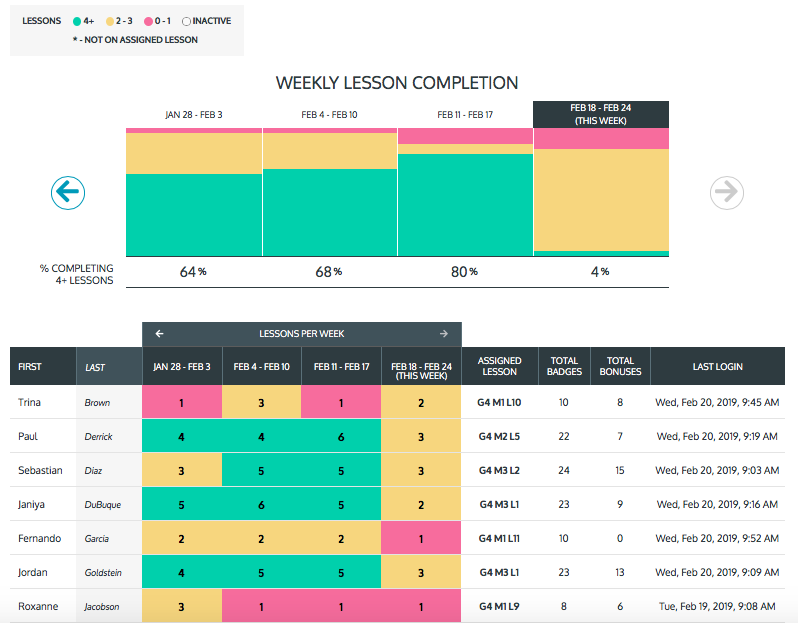
\includegraphics{images/class-report.png}

}

\caption{\label{fig-class-report}Sample Class Report}

\end{figure}%

A key feature of Zearn is its badge system, which tracks student
progress and motivates continued learning (see
Figure~\ref{fig-badges-screen}). Students earn badges upon mastery of
specific skills, providing a tangible representation of their
achievement. This system motivates students and provides teachers with
valuable data on student performance, informing their decision-making
process \citep{knudsen2020}. Zearn also incorporates notifications,
known as Tower Alerts, sent to teachers when a student struggles with a
specific concept. This feature allows teachers to provide timely support
and address learning gaps, enhancing the platform's capacity for
personalized learning.

\begin{figure}

\centering{


\includegraphics{images/badges.PNG}

}

\caption{\label{fig-badges-screen}Badge System for Student Achievement}

\end{figure}%

Another noteworthy aspect is the platform's professional development
component, which is available for schools with a paid account (see SI
for a sample training schedule). Teachers explore each unit or mission
through word problems, fluencies, and small group lessons, conducting
collaborative analysis of student work and problem-solving strategies.
This professional development revolves around each mission's big
mathematical idea, visual representations to scaffold learning, and
strategies to address unfinished learning from prior grades and
preparation for future learning \citep{morrison2019}.

The platform encapsulates a holistic methodology in mathematics
education, intertwining a hybrid curriculum that leverages print and
digital mediums, a rotational pedagogical model, targeted professional
development programs, and detailed analytics at the classroom and
institutional level to inform teaching and learning practices. This
integrated framework furnishes a rich repository of data for
comprehensive analysis. The variables delineated for investigation by
the Zearn consortium encompass a variety of dimensions: (1) teacher
engagement, quantified through a diverse set of actions; (2) student
achievement, denoted by variables such as lesson completion (i.e.,
``badges'' earned after each lesson is finished with full proficiency);
and (3) student struggles, monitored through variables such as ``tower
alerts''.

\subsection{Research Questions}\label{research-questions}

We propose the following research questions to explore the dynamics of
teacher behavior, the role of reinforcement learning in modeling these
behaviors, and the subsequent impact on student achievement. We hope to
shed light on the potential of reinforcement learning for understanding
human behavior in field data.

1. Characterizing Teacher Behavior: Can reinforcement learning models
fit teacher behavior better than a logistic regression model? Which
reinforcement learning model most accurately characterizes the behavior
of teachers in the context of Zearn Math? What insights about teacher
behavior do these differences in model fit bring?

2. Impact of RL Parameters on Teacher Behavior and Student Achievement:
How do the parameters of reinforcement learning models vary with teacher
behavior? What effects do these variations have on student achievement?

3. Influence of Teacher and School Background: How do factors such as
teacher background influence their adaptation to and implementation of
the Zearn Math curriculum? How can these factors be effectively
incorporated into the reinforcement learning model to provide a more
comprehensive understanding of teacher behavior and its impact on
student outcomes?

\section{Theory}\label{theory}

\subsection{Reinforcement Learning to Capture Patterns in Repeated
Behavior}\label{reinforcement-learning-to-capture-patterns-in-repeated-behavior}

In RL, an agent learns to make decisions over time to maximize a
cumulative reward. At the heart of RL is the concept of a policy, which
is a mapping from states to actions or, more commonly, a probability
distribution over actions \citep{sutton2018}. The agent's goal is to
learn an optimal policy, which maximizes the expected cumulative reward,
even when the parameters of the environment are not known a priori.

The application of RL in the context of education and teaching is not
new. One of the pioneers in the field of Markov decision processes,
Ronald Howard, attempted to apply his mathematical framework to
instruction theory as early as 1960 \citep{howard1960}. Later, in 1972,
Richard Atkinson proposed a theory of instruction that encapsulates the
key components of a Markov decision process, including states, actions,
transition probabilities, reward functions, and a time horizon
\citep{atkinson1972}. In Atkinson's framework, actions are instructional
activities (e.g., assigning problem sets) that can change a given state
(e.g., student learning level). These changes in states can yield
rewards minus the associated cost of the action. For example, a teacher
may be rewarded with an increase in the knowledge or skill of a student,
but such reward must be balanced with its associated effort (e.g., labor
cost). Atkinson and colleagues continued to test many parametrizations
of this idea, contributing significantly to the development of RL theory
in the context of education (see \citep{doroudi2019} for a full review).

More recently, RL models have been used in the psychology of habit to
explain learning and reward association. One common approach in human
studies is to apply the ``multi-armed bandit'' task. In this type of
experiment, participants are presented with multiple actions, each with
an unknown payoff. The subject's goal is to learn the best outcome
through trial and error. In the beginning, the reward-action
relationships are unknown, so the participant must explore or sample
each action \citep{sutton2018} . This exploration-exploitation trade-off
is a central theme in RL and has the potential to provide valuable
insights into how students learn and make decisions over time.

\subsection{Education production
function}\label{education-production-function}

Previous research has explored how teacher effort affects student
achievement. In particular, economists have studied the ``education
production function,'' in which educational outcomes are a function of
various inputs, including teacher effort, student effort, school
resources, and family background \citep{hedges1994}. This function
serves as a theoretical framework for understanding how different
factors contribute to educational achievement and how interventions can
be designed to improve outcomes.

One of the key inputs in the education production function is teacher
effort, as teachers play a crucial role in shaping students' learning
experiences and outcomes. Their effort, which encompasses their time,
energy, dedication, and instructional strategies, can significantly
influence students' academic achievement \citep{rivkin2005}. However,
measuring teacher effort and its impact on student outcomes can be
challenging due to the complex and multifaceted nature of teaching.

To address this challenge, researchers have employed various strategies
to identify the effects of teacher effort on student achievement. One
common approach is to manipulate the conditions under which teachers
operate, thereby changing the levels of teacher effort. For instance,
\citep{duflo2011} conducted a randomized controlled trial in Kenya to
examine the effects of tracking, a practice of grouping students based
on their ability levels. Tracking has been a prominent tool in the
sociology of education and assumes that teacher inputs will depend on
the ability level of the students. This tailoring of teaching strategies
and content potentially enhances the instructor's effectiveness.

However, traditional social science approaches to studying the education
production function often lack the flexibility to account for changes in
context and experience and individual-level differences . Reinforcement
learning (RL) offers a promising alternative approach. RL models
incorporate a flexibility term (i.e., a learning rate) that allows for
changes in behavior with experience and an exploration versus
exploitation term (e.g., inverse temperature) that captures individual
differences in decision-making strategies. Furthermore, the RL framework
inherently accounts for the process of learning about rewards, making it
a flexible and dynamic tool for studying teacher behavior
\citep{sutton2018}.

\subsection{Why Reinforcement
Learning?}\label{why-reinforcement-learning}

Reinforcement Learning (RL) presents a paradigm shift from models that
employ a static approach to link teacher efforts with student outcomes,
such as the education production function. RL embodies the flexibility
to adapt and evolve strategies over time. This dynamic framework
reflects the continuous learning process seen in biological systems and
has the potential to concretize the evolving nature of educational
interactions. In this study, our RL models position teachers as agents
who navigate their environment (i.e., the classroom) by acting based on
their observations and feedback. This process allows for a detailed
understanding of the interplay between teacher actions, the classroom
environment, and the outcomes of these interactions, as such:

\[
\text{Agent} \xrightarrow[\text{Actions}]{\text{Performs}} \text{Environment} \xrightarrow[\text{Observations, Rewards}]{\text{Provides}} \text{Agent}
\]

Further, RL algorithms also enable the modeling of individual teachers'
decision-making processes. This approach renders the creation of
detailed profiles for instructors, understanding how they adapt and
respond to various states and rewards within the educational setting.
The flexibility and robustness of RL make it an ideal tool for adapting
to changing learning environments and addressing individual teacher and
classroom needs. By incorporating a wide range of variables (i.e.,
states, actions, and rewards), RL models are customizable to diverse
educational contexts and objectives. They can also account for the
inherent uncertainties in teaching, guiding the formulation of optimal
decision-making strategies under uncertain conditions.

The analytical capabilities of RL extend to identifying variations in
teacher learning and behavior and how these differences influence
student outcomes. By estimating individual teacher parameters, RL
provides insights into aspects such as teacher flexibility, enabling
targeted interventions by policymakers to enhance educational outcomes.
Conducting ``counterfactual analyses'' opens avenues for innovative
educational interventions. Beyond immediate study goals, RL models hold
the potential for automating instructional decisions based on identified
patterns, potentially alleviating the workload on teachers and
optimizing the educational process.

\subsection{Q-Learning Model}\label{q-learning-model}

The Q-learning algorithm is the first class of models we employ to
elucidate decision-making dynamics within an interactive environment.
Q-learning involves the iterative refinement of Q-value functions, which
map an agent's actions in a given state to evolving expectations of
future rewards (analogous to subjective value or utility). This
methodological approach is closely related to the classic ``multi-armed
bandit'' problem, wherein the agent faces a finite set of choices (e.g.,
slot machines), each linked to a specific reward schedule, and aims to
identify the optimal action that maximizes returns. Learning in this
model depends on adjusting expectations to reduce the impact of
prediction errors (the ``surprise level,'' or the difference between
expected and realized outcomes), using the Bellman equation to update
Q-values iteratively \citep{rummery}. Through this iterative process,
the equation calculates the value of each state-action pair by combining
the immediate reward with the discounted value of subsequent optimal
state-action configurations. This model frames decision-making as a
result of accumulated experience and the anticipation of future rewards.
Note that this framework is considered a model-free reinforcement
learning algorithm, because it does not require a model of an
environment's stochastic transitions to approximate expected rewards
\citep{watkins1992}.

The Q-function, \(Q(s, a)\), is defined for all state-action pairs
\((s, a)\), where \(s\) is the state and \(a\) is the action. The
Q-function represents the expected return or future reward for taking
action \(a\) in state \(s\) following a certain policy \(\pi = \Pr(a)\).
The Q-function is updated iteratively using the Bellman equation as
follows:

\begin{equation}\phantomsection\label{eq-q-learn}{
Q_\text{new}(s, a) = Q(s, a) + \alpha \delta
}\end{equation}

where \(\alpha\) is the learning rate, which determines how much the
Q-value is updated based on \(\delta\), the reward prediction error. The
reward prediction error is the difference between the estimated Q-value
and the observed reward plus the discounted future Q-value. This error
is used to update the Q-value in the direction of the observed reward,
as follows:

\begin{equation}\phantomsection\label{eq-RPE}{
\delta = r + \gamma \max_{a'} Q(s', a') - Q(s, a)
}\end{equation}

where:

\begin{itemize}
\item
  \(r\) is the immediate reward received after taking action \(a\) in
  state \(s\),
\item
  \(\gamma\) is the discount factor,
\item
  \(s'\) is the new state after taking action \(a\),
\item
  \(a'\) is the action to be taken in the new state \(s'\),
\item
  \(s\) is the current state,
\item
  \(a\) is the action taken,
\item
  \(\max_{a'} Q(s', a')\) is the maximum reward that can be obtained in
  the next state \(s'\),
\item
  \(Q(s, a)\) is the current estimate of the Q-value for action \(a\) in
  state \(s\).
\end{itemize}

The Q-learning algorithm uses this update rule to learn the Q-function
and, hence, the optimal policy. The agent starts with an initial
Q-function (which can be arbitrary) and then updates the Q-values based
on the experiences it gathers from interactions with the environment.
The update rule is applied every time the agent transitions from a state
\(s\) to a state \(s'\) by taking an action \(a\) and receiving a reward
\(r\). The agent selects actions based on a policy function of the
Q-values. A common choice is the softmax action selection method, which
which chooses actions probabilistically based on their Q-values. The
probability of choosing a particular action is defined as follows:

\begin{equation}\phantomsection\label{eq-softmax}{
\Pr(a) = \frac{e^{Q(s, a)/\tau}}{\sum_{a'} e^{Q(s, a')/\tau}}
}\end{equation}

where:

\begin{itemize}
\item
  \(\Pr(a)\) is the probability of choosing action \(a\),
\item
  \(Q(s, a)\) is the Q-value of action \(a\) in state \(s\),
\item
  \(\tau\) is a parameter known as the temperature, which controls the
  level of exploration,
\item
  The denominator is the sum over all possible actions \(a'\) of the
  exponential of their Q-values divided by the temperature.
\end{itemize}

One possible interpretation of the temperature parameter \(\tau\) is the
control of the trade-off between exploration and exploitation. When
\(\tau\) is high, the agent explores more because the action
probabilities are more uniform. When \(\tau\) is low, the agent exploits
more because the action with the highest Q-value is more likely to be
chosen than the others. As the agent learns, it can be beneficial to
start with a high temperature to encourage exploration and then
gradually decrease it to favor the exploitation of the learned policy.

\subsubsection{State-Free vs.~State-Based
Models}\label{state-free-vs.-state-based-models}

So far, we have defined a state-based model that accounts for different
states of the environment into the Q-function. However, a special case
of the Q-learning model does not require a state space, prescribing only
an action-reward relationship, and the Q-value, \(Q(a)\), becomes a
function of the action alone. In our context, such an adaptation would
assume that the best action in one week is the best action at any other
week. This means a teacher learns the value of their action regardless
of the history of their classroom or students. Generally, this
assumption can be beneficial in scenarios where the state exerts minimal
influence on the outcome of the action or when the state is difficult to
define or observe \citep{sutton2018}. The Q-value update function,
therefore, simplifies to:

\begin{equation}\phantomsection\label{eq-state-free}{
Q(a) = Q(a) + \alpha \left[ r(a) - Q(a) \right]
}\end{equation}

where:

\begin{itemize}
\item
  \(Q(a)\) is the current estimate of the Q-value for action \(a\),
\item
  \(\alpha\) is the learning rate,
\item
  \(r(a)\) is the immediate reward received after taking action \(a\).
\end{itemize}

In this equation, the term in the brackets, \(r(a) - Q(a)\), is the
reward prediction error. It represents the difference between the
observed reward and the current estimate of the Q-value. The Q-value is
updated in the direction of this error, scaled by the learning rate
\(\alpha\).

\subsection{The Actor-Critic Model}\label{the-actor-critic-model}

For cases in which states do matter in teacher decisions, we choose a
model that divides the action selection and action evaluation tasks into
two components: the ``actor'' and the ``critic'' \citep{sutton2018b}.
This division theoretically allows for more efficient learning, as the
critic guides the actor's learning process.

The ``actor'' in this model selects actions based on a policy function,
denoted as \(\pi(a|s)\), which maps states to actions, determining the
probability of taking each action in each state. The actor aims to learn
an optimal policy that maximizes the expected cumulative reward. In our
setting, we set the policy as a softmax function over action
preferences:

\[
\pi(a|s) = \frac{e^{h(a, s)}}{\sum_{a'} e^{h(a', s)}}
\]

where \(h(a, s)\) is the preference for action \(a\) in state \(s\).

The ``critic,'' on the other hand, evaluates the actions taken by the
actor by learning a value function, denoted as \(V(s)\). Given the
actor's current policy, the critic estimates the expected cumulative
reward from each state. The critic's feedback, in the form of the value
function, guides the actor's learning. We update the value function
based on the Temporal Difference (TD) error, a measure of the difference
between the estimated and actual return:

\[
\delta = r + \gamma V(s') - V(s)
\]

where \(r\) is the reward, \(\gamma\) is the discount factor, \(s'\) is
the new state, and \(s\) is the current state.

This separation of action selection and evaluation distinguishes the
Actor-Critic model. In Q-learning, a single Q-function selects and
evaluates actions. Conversely, in the Actor-Critic case, the actor
updates its policy to increase the probability of actions that lead to
higher-than-expected returns and decrease the probability of actions
that lead to lower-than-expected returns.

\subsection{Applying RL Models to the Zearn
Context}\label{applying-rl-models-to-the-zearn-context}

In this study, we propose an application of the Reinforcement Learning
(RL) algorithms for modeling teacher decision-making within the Zearn
platform.

Consider a typical teaching scenario: the state is the students' current
progress in the class, and the actions are a range of pedagogical
strategies, such as assigning additional practice, providing
personalized feedback, or adjusting lesson plans. Some relevant reward
variables include improved student performance, increased student
engagement, or reduced learning gaps.

In the Zearn context, we define the decision process as follows:

\begin{enumerate}
\def\labelenumi{\arabic{enumi}.}
\item
  Agents are the teachers.
\item
  Actions include the choice of specific pedagogical strategies.
\item
  The environment is the Zearn platform with its students.
\item
  The state is the week-over-week change in student performance and/or
  struggle.
\item
  The reward is a linear function of student performance.
\end{enumerate}

Mathematically mapping the agent-environment interaction is flexible,
with many models potentially satisfying our initial assumptions. We
approach this problem as a competition of models, selecting a set of
models applicable to our setting, fitting them to the data, and
comparing their performances.

\section{Material and Methods}\label{material-and-methods}

To accurately capture the intricate dynamics present within our data, we
explored a large set of candidate models, progressively escalating in
complexity, as shown in Table~\ref{tbl-methods}. This methodological
triangulation enabled us to refine our data processing, analysis, and
interpretation methods, effectively addressing the drawbacks of relying
solely on one analytical approach. Through this rigorous methodology,
our goal was to strengthen the reliability of our findings and offer a
detailed understanding of the underlying behavioral patterns.

\begin{longtable}[]{@{}
  >{\raggedright\arraybackslash}p{(\columnwidth - 4\tabcolsep) * \real{0.1561}}
  >{\raggedright\arraybackslash}p{(\columnwidth - 4\tabcolsep) * \real{0.4509}}
  >{\raggedright\arraybackslash}p{(\columnwidth - 4\tabcolsep) * \real{0.3873}}@{}}
\caption{Analytical steps employed in the
study.}\label{tbl-methods}\tabularnewline
\toprule\noalign{}
\begin{minipage}[b]{\linewidth}\raggedright
\textbf{Step}
\end{minipage} & \begin{minipage}[b]{\linewidth}\raggedright
\textbf{Method}
\end{minipage} & \begin{minipage}[b]{\linewidth}\raggedright
\textbf{Software/Tools}
\end{minipage} \\
\midrule\noalign{}
\endfirsthead
\toprule\noalign{}
\begin{minipage}[b]{\linewidth}\raggedright
\textbf{Step}
\end{minipage} & \begin{minipage}[b]{\linewidth}\raggedright
\textbf{Method}
\end{minipage} & \begin{minipage}[b]{\linewidth}\raggedright
\textbf{Software/Tools}
\end{minipage} \\
\midrule\noalign{}
\endhead
\bottomrule\noalign{}
\endlastfoot
Data Preprocessing & Cleaning, normalization & R
\citep{rcoreteam2024} \\
Dimensionality Reduction & Principal Component Analysis (PCA),
Non-negative Matrix Factorization (NMF) & Python (\texttt{scikit-learn})
\citep{pedregosa2011} \\
Feature Selection & Regression analysis & R (\texttt{fixest} package)
\citep{berge2018} \\
Analytical Methods & Q-learning, Actor-Critic Model Estimation & R,
Matlab (\texttt{CBM} package for Laplace approximation)
\citep{piray2019} \\
Statistical Analysis & Hierarchical Bayesian Inference & Matlab
(\texttt{CBM} package for expectation-maximization algorithm) \\
Model Evaluation & Hetereogeneity analyses of model performance across
teachers & R \\
\end{longtable}

\subsection{Data}\label{data}

The data from the Zearn platform follows a time-series structure,
spanning across an academic year, with the unit of analysis being the
classroom-week. This level of granularity enables us to capture the
temporal dynamics of teacher-student interactions and their subsequent
influence on student achievement. In particular, we can model the
decision-making process of teachers as they allocate their time and
effort on the Zearn platform weekly and how these decisions translate
into student outcomes, measured by the completion of lessons or
``badges.''

Zearn provided administrative data for teachers and students. Teacher
activity is time-stamped to the second and includes the time spent on
the platform and specific actions taken. On the other hand, student data
is aggregated at the classroom-week level due to data privacy
considerations. This aggregation included a variety of potentially
interesting variables capturing student achievement (e.g., student
lesson completion or ``badges'') and level of student struggle (e.g.,
tower alerts). These variables offer a comprehensive view of the
dynamics of teacher-student interactions on the Zearn platform.

\begin{longtable}{l|rrrr}

\caption{\label{tbl-summary}Summary statistics by school, detailing the
number of teachers, total students, and weeks of active engagement.}

\tabularnewline

\toprule
\multicolumn{1}{l}{} & Mean & Standard Deviation & Minimum & Maximum \\ 
\midrule\addlinespace[2.5pt]
Teachers & $29.14$ & $579.30$ & $1$ & $19,687$ \\ 
Students & $268.46$ & $279.56$ & $0$ & $3,289$ \\ 
Weeks & $24.12$ & $12.54$ & $1$ & $51$ \\ 
\bottomrule

\end{longtable}

The dataset includes 31046 classrooms and 19689 educators, with an
average of 17.6 students per classroom. Table~\ref{tbl-summary} provides
a snapshot of the schools' characteristics and reveals a broad spectrum
of Zearn's user demographics including the average number of teachers,
students, and weeks of data per school. The bimodal distribution of
weekly data per classroom, as showcased in
Figure~\ref{fig-classroom-weeks}, reveals that some classrooms have less
than 3 to 4 months of data. The classrooms with less than 16 weeks of
data are color-coded in red. The pattern of student logins over time,
particularly around significant holidays, as seen in
Figure~\ref{fig-logins-week}, underscore the temporal fluctuations in
platform engagement.

\begin{figure}

\centering{

\includegraphics{zearn_files/figure-pdf/fig-classroom-weeks-1.pdf}

}

\caption{\label{fig-classroom-weeks}Histogram of number of weeks of data
per classroom. A bimodal distribution highlights the majority of
classrooms with data spanning over 50 weeks. A smaller but significant
subset of classrooms have less than 18 weeks of data. The dashed line
acts as a threshold that excludes a notable segment of classrooms from
further analysis. The lack of data between these two peaks suggests
distinct patterns of usage---some classrooms consistently use the
platform throughout the academic year, while others show sporadic
engagement, possibly reflecting trial periods or intermittent usage.}

\end{figure}%

\begin{figure}

\centering{

\includegraphics{zearn_files/figure-pdf/fig-logins-week-1.pdf}

}

\caption{\label{fig-logins-week}Total number of student logins over
time. The chart depicts the connection between academic schedules and
platform engagement. Each bar represents a week, revealing peaks
coinciding with active school weeks and troughs aligning with holiday
periods (e.g., Thanksgiving and Christmas).}

\end{figure}%

\subsubsection{Geographic Context and
Distribution}\label{geographic-context-and-distribution}

Our investigation encompasses a diverse range of Louisiana schools. This
region presents a distinct educational landscape and widespread adoption
of the Zearn platform across its schools. Figure~\ref{fig-teachers-map}
maps the distribution of teachers engaged with Zearn across Louisiana's
parishes, highlighting areas with pronounced clusters of active
teachers. The map also marks the top five cities leading in Zearn
adoption among teachers.

\begin{figure}

\centering{

\includegraphics{zearn_files/figure-pdf/fig-teachers-map-1.pdf}

}

\caption{\label{fig-teachers-map}Geographic distribution of Zearn
teachers across Lousiana parishes. The color gradient indicates the
density of teachers, with darker hues representing a greater number of
educators using Zearn. The top five cities where Zearn is most prominent
are identified and labeled.}

\end{figure}%

To enhance our analysis, we have included the socioeconomic profile
detailed in Figure~\ref{fig-income-dist}. The distributions of median
poverty and income levels highlight the heterogeneity in our data and
the potential for understanding the impact of socioeconomic factors on
the educational landscape.

\begin{figure}

\begin{minipage}{0.50\linewidth}

\centering{

\includegraphics{zearn_files/figure-pdf/fig-income-dist-1.pdf}

}

\subcaption{\label{fig-income-dist-1}School Poverty Distribution}

\end{minipage}%
%
\begin{minipage}{0.50\linewidth}

\centering{

\includegraphics{zearn_files/figure-pdf/fig-income-dist-2.pdf}

}

\subcaption{\label{fig-income-dist-2}Median Income Distribution}

\end{minipage}%

\caption{\label{fig-income-dist}Distributions of School Socioeconomic
Profiles. The first graph shows school poverty levels based on the
eligibility for free or reduced-price lunch (FRPL), a proxy for
low-income student concentration. Schools are categorized by the
percentage of eligible students: low-poverty (0-40\%), mid-poverty
(40-75\%), and high-poverty (over 75\%). The second graph depicts the
median income distribution within the school districts.}

\end{figure}%

\subsubsection{Preprocessing and Exclusion
criteria}\label{preprocessing-and-exclusion-criteria}

In order to model interesting behavioral patterns, we focus our analysis
on the teachers who most likely take advantage of a wide range of
resources on the platform. Thus, we select teachers who consistently use
the platform and work in traditional school settings. To achieve this,
the raw data underwent rigorous preprocessing to ensure its suitability
for analysis. This process included performing log transformations on
our variables of interest (i.e., minutes, badges, and tower alerts) to
normalize their distributions. Given the diverse user base of Zearn, we
applied specific exclusion criteria to select teachers who most likely
representat traditional classroom settings with consistent platform
utilization. We selected virtual classrooms with at least five active
students weekly, filtering out parents or tutors who may use Zearn
outside the classroom setting. We removed teachers with more than four
classrooms and those who logged in for less than 16 weeks. We excluded
classrooms in the 6th to 8th grades, as they represent only a small
proportion of our dataset. This deletion ensures a focus on traditional
school settings, minimizing bias from teachers and schools that have not
used Zearn consistently.

Table~\ref{tbl-classroom-summary} summarizes the refined dataset,
providing a snapshot of the key variables of interest. Their means and
standard deviations (SD) are computed for each grade level and overall
(across all grades).

\begin{longtable}{l|rrrr}

\caption{\label{tbl-classroom-summary}Classroom engagement by grade
level. Means (standard deviations) of minutes and badges per student,
Tower Alerts per lesson completion, and teacher engagement minutes.}

\tabularnewline

\toprule
\multicolumn{1}{l}{} & Minutes & Badges & Tower Alerts & Teacher Minutes \\ 
\midrule\addlinespace[2.5pt]
Overall, N = 135,784 & 81 (56) & 2.43 (1.91) & 0.47 (0.81) & 84 (149) \\ 
Kindergarten, N = 7,486 & 41 (34) & 4.44 (3.59) & 0.05 (0.35) & 21 (46) \\ 
1st, N = 21,126 & 80 (51) & 2.50 (1.64) & 0.40 (0.45) & 65 (107) \\ 
2nd, N = 26,424 & 84 (55) & 2.46 (1.67) & 0.36 (0.59) & 70 (122) \\ 
3rd, N = 26,316 & 84 (55) & 2.42 (1.71) & 0.44 (0.60) & 100 (175) \\ 
4th, N = 27,048 & 84 (59) & 2.13 (1.74) & 0.56 (0.81) & 100 (169) \\ 
5th, N = 27,384 & 84 (59) & 2.10 (1.66) & 0.71 (1.28) & 101 (165) \\ 
\bottomrule

\end{longtable}

\subsubsection{Operationalizing Actions, Rewards, and
States}\label{operationalizing-actions-rewards-and-states}

In analyzing Zearn data spanning an entire academic year, we must
establish a framework for input (actions), output (rewards), and,
optionally, state variables for state-based RL models. In this
framework, teacher activities drive the educational process, student
achievements result from these efforts, and the constantly changing
educational environment represents the states. The following sections
will further explore potential actions, rewards, and states in our
dataset.

\paragraph{Teacher Actions}\label{teacher-actions}

Teacher actions encompass a broad spectrum, from platform log-ins to
resource downloads and specific instructional activities.
Simultaneously, student engagement is captured through metrics such as
lesson completions (badges earned) and time spent logged in.
Table~\ref{tbl-teacher-variables} provides a list of the actions
available in the data.

\begin{longtable}[]{@{}
  >{\raggedright\arraybackslash}p{(\columnwidth - 2\tabcolsep) * \real{0.2125}}
  >{\raggedright\arraybackslash}p{(\columnwidth - 2\tabcolsep) * \real{0.7875}}@{}}
\caption{Catalog of Teacher Activities. This table presents teachers'
actions, including curriculum engagement, downloads of pedagogical
materials, and completion of various interactive components within the
Zearn educational platform.}\label{tbl-teacher-variables}\tabularnewline
\toprule\noalign{}
\begin{minipage}[b]{\linewidth}\raggedright
\textbf{Variable}
\end{minipage} & \begin{minipage}[b]{\linewidth}\raggedright
\textbf{Description}
\end{minipage} \\
\midrule\noalign{}
\endfirsthead
\toprule\noalign{}
\begin{minipage}[b]{\linewidth}\raggedright
\textbf{Variable}
\end{minipage} & \begin{minipage}[b]{\linewidth}\raggedright
\textbf{Description}
\end{minipage} \\
\midrule\noalign{}
\endhead
\bottomrule\noalign{}
\endlastfoot
PD Course Guide Download \citep{zearnaa, zearnab} & Detailed agenda for
Professional Development (PD) courses focusing on classroom
implementation, leadership, supporting diverse learners,using data to
inform teaching practices, and accelerating student learning. \\
PD Course Notes Download \citep{zearnaa, zearnab} & Professional
development session notes offering insights into effectively using
Zearn's curriculum. \\
Curriculum Map Download \citep{zearna} & Detailed outline of learning
objectives and content. Presents a sequence of interconnected math
concepts across grades, aligning with states' instructional
requirements. \\
Assessments Download \citep{zearnb} & Assessments to evaluate student
understanding of the material, including ongoing formative assessments,
digital daily checks, and paper-based unit assessments. \\
Assessments Answer Key Download \citep{zearnc} & Solutions for
assessments to aid in grading and feedback. Provides detailed rubrics
for mission-level assessments. \\
Elementary Schedule Download \citep{zearne} & A recommended schedule for
elementary school-level Zearn curriculum activities to guide daily and
weekly instructional planning, ensuring comprehensive coverage of
curriculum content. \\
Grade Level Overview Download \citep{zearnf} & Provides a summary of
learning objectives, pacing guidance, key grade-level terminology, a
list of required materials, and details on the standards covered by each
lesson. \\
Kindergarten Schedule Download \citep{zearng} & Recommended schedules
for Kindergarten, supporting structured instruction planning. \\
Kindergarten Mission Download \citep{zearnh} & Details interactive
activities focused on kindergarten-level concepts and their learning
objectives. \\
Mission Overview Download \citep{zearnf} & Outlines a mission's (i.e.,
learning module) flow of topics, lessons, and assessments; highlights
foundational concepts introduced earlier; lists recently introduced
terms and required materials for teacher-led instruction. \\
Optional Homework Download \citep{zearnj} & Assignments for additional
practice, enhancing student learning outside of class. \\
Optional Problem Sets Download \citep{zearnk} & Exercises for extra
practice, tailored to reinforce lesson concepts. \\
Small Group Lesson Download \citep{zearnl} & Lessons designed for
small-group engagement. \\
Student Notes and Exit Tickets Download \citep{zearnz, zearny} & Student
notes supplement digital lessons with paper-and-pencil activities. Exit
tickets are lesson-level assessments for teachers to monitor daily
learning. \\
Teaching and Learning Approach Download \citep{zearnn} & Resources
outlining Zearn's pedagogical methods. \\
Whole Group Fluency Download \citep{zearno} & Lesson-aligned practice
activities to build math fluency through whole-class engagement. \\
Whole Group Word Problems Download \citep{zearnl} & Word problem-solving
activities intended for collaborative, whole-class engagement. \\
Fluency Completed \citep{lesson-a} & Indicates teacher completed a
fluency activity, typically given to students before their daily digital
lessons. \\
Guided Practice Completed \citep{zearnr} & Indicates teacher completed a
guided practice segment, where students learn new concepts. These
include videos with on-screen teachers, interactive activities, and
paper-and-pencil Student Notes. \\
Kindergarten Activity Completed \citep{zearns} & Indicates teacher
completed an activity within the Kindergarten curriculum. \\
Number Gym Activity Completed \citep{zearnt} & Indicates teacher
completed a Number Gym, an individually adaptive activity that builds
number sense, reinforces previously learned skills, and addresses areas
of unfinished learning. \\
Tower Completed \citep{zearnu} & Indicates teacher completed a Tower of
Power, an activity that requires full mastery of lesson objectives and
that students must complete independently. \\
Tower Struggled \citep{zearnac} & Indicates teacher committed a mistake
when engaging with the Tower of Power activity in a student role,
triggering a ``boost'' (scaffolding remediation). \\
Tower Stage Failed \citep{zearnad} & Indicates teacher received three
consecutive ``boosts'' due to repeated errors when engaging with the
Tower of Power in a student role. \\
\end{longtable}

\paragraph{Reward and State Variables}\label{reward-and-state-variables}

Reward and state variables in Reinforcement Learning (RL) models capture
the dynamics of the environment in which learning and actions occur. The
Zearn platform captures these variables from student activity and
performance data, providing a quantifiable snapshot of classroom
engagement and learning challenges. The student variables in our data
are:

\begin{enumerate}
\def\labelenumi{\arabic{enumi}.}
\item
  ``Active Students'' directly measures classroom engagement,
  representing the number of students actively logging in to complete
  digital lessons within a given week \citep{zearn2022}.
\item
  ``Student Logins'' functions as an attendance roster, tallying the
  frequency of students entering the platform, potentially serving as an
  engagement metric \citep{zearnaf}.
\item
  ``Badges (on grade)'' and ``Badges'' per active user metrics offer
  insights into the level of curriculum mastery. They reflect the number
  of new lessons completed weekly at students' grade level and in
  general. Accumulating badges can serve as a reward signal in an RL
  model, indicating students' progress and pace through the curriculum
  \citep{zearnae}.
\item
  ``Minutes per active student'' variable measures students' time on the
  platform, potentially correlating with their focus and learning
  progress. Once routines are established, teachers can use this metric
  to monitor whether students meet their expected weekly minutes
  \citep{zearn2022}.
\item
  ``Tower Alerts'' signal instances when students repeatedly encounter
  difficulties within the same lesson, prompting the platform to notify
  teachers. In the context of RL models, Tower Alerts could be viewed as
  a negative reinforcement signal, highlighting areas where students may
  require additional support or intervention to improve learning
  outcomes \citep{zearnad}.
\end{enumerate}

\subsubsection{Dimensionality Reduction}\label{dimensionality-reduction}

While comprehensive, directly using the available variables presents
certain challenges:

\begin{enumerate}
\def\labelenumi{\arabic{enumi}.}
\tightlist
\item
  \textbf{Complexity}: The sheer number of available variables
  complicates the identification of meaningful patterns and
  relationships.
\item
  \textbf{Dimensionality}: The high-dimensional nature of the data risks
  diluting important signals due to the ``curse of
  dimensionality.''\footnote{Richard Bellman coined this phrase to
    describe the challenge of optimizing a control process by searching
    over a discrete multidimensional grid, where the number of grid
    points increases exponentially with the number of dimensions. He
    wrote: ``In view of all that we have said in the foregoing sections,
    the many obstacles we appear to have surmounted, what casts the pall
    over our victory celebration? It is the curse of dimensionality, a
    malediction that has plagued the scientist from the earliest days''
    \citep{bellman2015adaptive}.}
\item
  \textbf{Interpretability}: Directly interpreting the impact of
  specific actions or behaviors on outcomes can be obscured by the
  intertwined nature of the data.
\end{enumerate}

Given these considerations, we avoid relying solely on single, discrete
variables and employ dimensionality reduction techniques.

By reducing the data to a manageable number of components, we can more
readily identify underlying patterns of behavior and interaction.
Components generated through this technique provide a distilled
representation of the data, where each one reflects a combination of
behaviors or activities with a potential thematic linkage. To achieve
this, we applied Principal Component Analysis (PCA) and Nonnegative
Matrix Factorization (NMF) techniques. We then used the results to
define action, reward, and state variables rather than using individual
metrics.

PCA is our first methodological choice. It is widely utilized but
assumes data normality \citep{jolliffe2016} and maximizes variance
explained, potentially overlooking subtle relationships between
variables. Consequently, we also employ NMF, which, by contrast, imposes
a non-negativity constraint and is more closely related to clustering
algorithms, creating a more interpretable, sparse representation of
behaviors \citep{ding2005, lee1999}. This technique is particularly
advantageous for data representing counts or frequencies. By trying
different techniques, we can explore these trade-offs and discover the
reduced-dimension representation best suited to our specific dataset and
research questions.

First, we standardized the dataset by z-scoring the variables of
interest at the school level (using school-wide means and standard
deviations). We performed PCA and NMF, and we evaluated the data's
reconstruction accuracy and cluster separation using, respectively, the
sum of squared residuals (a measure of the difference between the
original data and the reconstructed data) and silhouette scores (a
measure of how similar an object is to its cluster compared to other
clusters \citep{rousseeuw1987}).

We calculate the silhouette score with the formula
\((b - a) / \max(a, b)\), where \(a\) is the average distance within a
cluster and \(b\) is the average distance to the nearest neighboring
cluster. This score ranges from -1 to 1, with higher values indicating a
data point is well-matched to its cluster and poorly matched to
neighboring clusters.

Note that our chosen RL models require discreet action variables. Thus,
we choose to split teacher actions into binary variables, following a
median split.

\paragraph{Nonnegative Matrix Factorization (NMF)
Methodology}\label{nonnegative-matrix-factorization-nmf-methodology}

Let the original matrix (\(\mathbf{V}\)) be a detailed description of
all the teachers' (or students') behaviors. Each row in the matrix
represents a unique teacher-week (or classroom-week), and each column
represents a specific behavior or action. The entry in a specific row
and column corresponds to the frequency of that behavior for that
particular teacher-week (or classroom-week). We then estimate
\(\mathbf{V} \simeq \mathbf{W}\mathbf{H}\), such that we minimize the
following:

\[
\left\| \mathbf{V} - \mathbf{W}\mathbf{H} \right\| , \mathbf{W} \geq 0, \mathbf{H} \geq 0.
\]

We used two different loss functions (Frobenius norm and
Kullback-Leibler divergence) and two different initialization methods
(nonnegative double singular value decomposition (NNDSVD) and NNDSVD
with zeros filled with the average of the input matrix (NNDSVDA)). The
resulting matrices are:

\begin{enumerate}
\def\labelenumi{\arabic{enumi}.}
\tightlist
\item
  Basis Matrix (\(\mathbf{W}\)): This matrix represents underlying
  behavior patterns. Each column is a ``meta-behavior'' or a group of
  behaviors occurring together.
\item
  Mixture Matrix (\(\mathbf{H}\)): This matrix shows the extent to which
  each ``meta-behavior'' is present in each teacher-week (or
  classroom-week). Each entry in this matrix represents the contribution
  of a ``meta-behavior'' to a particular behavior present in the data.
\end{enumerate}

These matrices can reveal underlying patterns of behaviors (from the
basis matrix) and how these patterns are mixed and matched in different
teachers (from the mixture matrix). It allows us to assess the method's
performance under varying configurations, with the sum of squared
residuals and silhouette scores for comparison.

One desirable feature of NMF is that it produces sparse components. In
most cases, a median split is equivalent to giving a value of 1 to any
positive entry. This sparsity makes the results more interpretable.

\subsection{Analytical Methods}\label{analytical-methods}

\subsubsection{Feature Selection}\label{feature-selection}

In order to pre-select the most appropriate action, reward, and state
variables, we used a panel logistic regression model inspired by dynamic
analysis \citep{lau2005}. This approach acted as a filter to capture the
action-reward (or action-reward-state) configurations displaying
characteristics reminiscent of reinforcement learning (RL). We followed
four criteria: a) the influence of consistent rewards on the propensity
of actions being repeated, b) the immediate impact of states on action
selection, c) the strategic role of actions in navigating towards
desirable states, and d) the identification of action auto-correlation
as an indicator of incremental learning processes.

Unlike \citep{lau2005}, our model is not limited to the lagged effects
of actions and rewards. We also capture action-reward interactions and
the contemporaneous influence of states on actions. The general model
formulation for state-free and state-based scenarios is as follows:

\paragraph{State-Free Model}\label{state-free-model}

\begin{align*}
\text{Action}_t =& \ \sum_{i=1}^{L} \left( \beta_{i} \text{Reward}_{t-i} + \gamma_i \text{Action}_{t-i} + \sum_{j=i}^{L} \delta_{ij} (\text{Reward}_{t-i} \times \text{Action}_{t-j}) \right) \\
& + \mu_{\text{Teacher}} + \lambda_{\text{Week}} + \epsilon_t 
\end{align*}

\paragraph{State-Based Model}\label{state-based-model}

\begin{align*}
\text{Action}_t =& \ \sum_{i=1}^{L} \left( \beta_{i} \text{Reward}_{t-i} + \gamma_i \text{Action}_{t-i} + \sum_{j=i}^{L} \delta_{ij} (\text{Reward}_{t-i} \times \text{Action}_{t-j}) \right) \\
& + \phi \text{State}_{t-1} + \psi (\text{State}_{t-1} \times \text{Action}_{t-2}) + \mu_{\text{Teacher}} + \lambda_{\text{Week}} + \epsilon_t
\end{align*}

where \(\text{Action}_t\) denotes the binary outcome at time \(t\),
\(\text{Reward}_{t-i}\) and \(\text{Action}_{t-i}\) represent the reward
and action variables lagged by \(i\) periods, and \(L\) is the maximum
lag considered. \(\mu_{\text{Teacher}}\) and \(\lambda_{\text{Week}}\)
represent fixed effects for teachers and weeks, respectively.

\paragraph{Varying Coefficients Model}\label{varying-coefficients-model}

We used a varying coefficients model to capture individual teacher
effects on the dynamics between rewards, actions, and states. The model
is specified as follows:

\begin{align*}
\text{Action}_{kt} =& \ \sum_{i=1}^{L} \left( \beta_{ki} \text{Reward}_{k, t-i} + \gamma_{ki} \text{Action}_{k, t-i} + \sum_{j=i}^{L} \delta_{kij} (\text{Reward}_{k, t-i} \times \text{Action}_{k, t-j}) \right) \\
& + \phi_k \text{State}_{kt} + \psi_k (\text{State}_{kt} \times \text{Action}_{k, t-1}) + \mu_k + \lambda_{\text{Week}} + \epsilon_{kt}
\end{align*}

where \(\beta_{ki}\), \(\gamma_{ki}\), and \(\delta_{kij}\) represent
the reward, action, and their interaction coefficients that vary by
teacher; \(\phi_k\) and \(\psi_k\) are the effects for the state and the
interaction between state and lagged action, respectively; and \(\mu_k\)
and \(\lambda_{\text{Week}}\) are fixed effects for teachers and weeks,
respectively.

Herein, the interaction between lagged rewards and actions aimed to
capture the reinforcement aspect (a), where prior rewards enhance the
likelihood of repeating specific actions. Including current state
variables addressed (b) and examining how present educational contexts
inform action choices. The interaction between current states and lagged
actions encapsulated (c) that actions are deliberately chosen to
navigate towards or sustain preferable educational states. Lastly,
considering lagged rewards alone, we sought to elucidate (d) the
phenomenon where past successes influence future endeavors, indicative
of a learning trajectory.

To operationalize these models, we constructed lagged versions of the
variables, extending up to six weeks to determine the optimal lag. This
lag value captured how far back rewards and past actions influenced
teacher behavior.

Two types of metrics anchored model selection. First, we split the data
into training (80\%) and testing (20\%) subsets. Then, we evaluated
model fit and predictive accuracy using the Bayesian Information
Criterion (BIC) and the Out-of-Sample fit, gauged through the Area Under
the Receiver Operating Characteristic curve (AUC). As such, we balanced
model parsimony with predictive power. Second, we aimed to delineate
which regression coefficients most closely embodied RL-like dynamics. We
focused on a) variables that consistently enhanced action probability in
response to rewards (i.e., positive coefficient for the state-reward
interaction), b) actions that changed according to a given state, c)
actions chosen to achieve desired states (i.e., significant coefficient
for the action-state interaction), and d) demonstrate action
auto-correlation.

\subsubsection{Reinforcement Learning Model
Estimation}\label{reinforcement-learning-model-estimation}

For the initial model selection, we fit the data from 295 classrooms due
to computational constraints. After selecting the optimal model, we
scale up the analysis to include all classrooms.

\paragraph{State-Free Q-Learning
Model}\label{state-free-q-learning-model}

We use a state-free version of the Q-learning model to predict the
actions of teachers based on their past actions and the rewards they
received. Thus, the Q-value for action \(a\) is updated based on the
reward prediction error \(\delta\):

\[
Q_{t+1}(a) = Q_{t}(a) + \alpha \left( \gamma (\text{Reward}_t - \text{cost}(a)) - Q_{t}(a) \right)
\]

where

\begin{itemize}
\tightlist
\item
  \(\alpha\) is the learning rate,
\item
  \(\gamma\) is the discount rate,
\item
  \(\text{Badges}_t\) is the immediate reward received after taking
  action \(a\) in state \(s\),
\item
  \(\text{cost}(a)\) is the estimated cost associated with action \(a\),
\item
  \(Q_{t}(a)\) is the estimate of the Q-value for action \(a\) at time
  \(t\).
\end{itemize}

The probability of choosing a particular action is determined by the
softmax function and is defined as follows:

\[
\Pr_t(a) = \frac{1}{1+e^{-\tau Q_{t}(a)}}
\]

where:

\begin{itemize}
\tightlist
\item
  \(\Pr_{t}(a)\) is the probability of choosing action \(a\) at time
  \(t\),
\item
  \(\tau\) is the temperature parameter.
\end{itemize}

We interpret each of these parameters as follows:

\begin{itemize}
\item
  Cost: The perceived effort or inconvenience associated with the
  action, such as the effort required to complete a particular task or
  the inconvenience of deviating from a preferred teaching method.
\item
  Learning rate (\(\alpha\)): The extent to which the newly acquired
  information will override the old information. A factor of 0 will make
  the agent not learn anything.
\item
  Discount rate (\(\gamma\)): The degree to which future rewards are
  discounted compared to immediate rewards. A high discount rate means
  that future rewards are considered almost as valuable as immediate
  rewards, which encourages long-term planning. A low discount rate
  means that immediate rewards are much more valuable than future
  rewards, which encourages short-term thinking.
\item
  Inverse temperature (\(\tau\)): The degree of randomness in the choice
  behavior. A high inverse temperature means that the agent is more
  likely to choose the action with the highest expected reward, while a
  low inverse temperature means that the agent is more likely to choose
  actions randomly. This parameter can be interpreted as a measure of
  the agent's confidence in its Q-values, reflecting the trade-off
  between exploration (trying out new actions) and exploitation
  (sticking to known beneficial actions).
\end{itemize}

\paragraph{The Actor-Critic Model}\label{the-actor-critic-model-1}

In the Actor-Critic model, we update the value function, parameterized
by weights \(w\), and the policy function, defined by the parameter
\(\theta\). The model's update mechanism is minimizing the prediction
error (\(\delta\)), which drives adjustments to both the actor and
critic components. The equations for updating the weights and policy are
as follows:

\[
w_{t+1} = w_{t} + \alpha_{v} \cdot \delta \cdot S_{t}
\]

\[
\theta_{t+1} = \theta_{t} + \alpha_{\pi} \cdot \delta \cdot S_{t}
\]

where \(w_{t}, \theta_{t}\) are the vectors of policy and value weights,
respectively, for action \(a\), and \(S_{t}\) is a vector that
characterizes the current state, defined as
\(S_{t} = \begin{bmatrix} 1 \\ \text{State Variable}_{t} \end{bmatrix}\).

We define the parameterized policy as
\(\Pr_{t}(a)=\text{Logit}^{-1}(\theta_{t} \cdot S_{t})\), the values of
each state as \(v(S_{t},a) = w_{t} \cdot S_{t}\), and prediction error
\(\delta\) as the difference between the actual outcome and the
estimated value of the state-action pair:

\[
\delta = (\text{Reward}_{t} - \text{cost}(a)) - \left( \gamma v(S_{t},a) - v(S_{t+1},a) \right)
\]

\paragraph{Hybrid Models}\label{hybrid-models}

The hybrid models maintain parallel estimations of two models (Logistic
regression, Q-learning, or Actor-Critic), combining them to estimate
action selection. This integration is achieved through a weighting
scheme that balances the contributions of each model. Specifically, the
probability of selecting action (\(a\)) at time (\(t\)), denoted
(\(\Pr_t(a)\)), is calculated through a linear combination of the
softmax outputs of the selected models. This integration uses a
weighting parameter (\(\lambda\)), which adjusts the relative influence
of each model and is formulated as:

\[
\Pr_t(a) = \lambda \Pr_t(a)_{\text{Model 1}} + (1-\lambda) \Pr_t(a)_{\text{Model 2}},
\]

\subsection{Model Estimation}\label{model-estimation}

We adopt the Hierarchical Bayesian Inference (HBI) framework, as
described by \citep{piray2019a}, to assess the fitness of our RL models
and estimate their respective parameters across subjects. This approach
uses Laplace approximations for efficient computation of posteriors by
approximating the integrals involved in Bayesian inference.
Subsequently, it leverages population-level distributions to refine
individual parameter variation. Within this framework, we assume that
for any given model \(k\) and subject \(n\), the individual parameters
(\(h_{k,n}\)) are normally distributed across the population with
\(p(h_{k,n}) = N(h_{k,n} | \mu_k, V_k)\), where \(\mu_k\) and \(V_k\)
represent the mean and variance of the prior distribution over
\(h_{k,n}\), respectively.

We use an expectation-maximization algorithm, iteratively performing the
following two steps:

\begin{enumerate}
\def\labelenumi{\arabic{enumi}.}
\tightlist
\item
  Expectation Step: The algorithm calculates a posteriori estimates of
  the individual parameters (\(h_{k,n}\)) based on the existing
  group-level distributions.
\item
  Maximization Step: The algorithm refines the group-level parameters
  (\(\mu_k\) and \(V_k\)) using current individual parameter estimates.
  The updated mean group parameter \(\mu_k\) is computed as the average
  of subject-level mean estimates (\(\theta_{k,n}\)) across all
  subjects, conforming to \(\mu_k = \frac{1}{N}\sum_{n}\theta_{k,n}\),
  where \(N\) is the total number of subjects.
\end{enumerate}

With this approach, we can estimate the log-likelihood for each
subject's data, given the proposed models and parameter estimates.
Recognizing the constraint of normality, we transform constrained
parameters (e.g., the learning rate and discount factor in the
Q-learning model). For parameters within a (0,1) interval, we use the
inverse logit function, \(\text{Logit}^{-1}\). Parameters like
temperature and costs, which are intrinsically non-negative, undergo an
exponential transformation to accord with the presumed normality in
their logarithmic space.

The parameters estimated for each model are as follows:

\begin{enumerate}
\def\labelenumi{\arabic{enumi}.}
\tightlist
\item
  Q-learning:

  \begin{itemize}
  \tightlist
  \item
    Learning Rate: \(\text{Logit}^{-1}(\alpha)\)
  \item
    Discount Rate: \(\text{Logit}^{-1}(\gamma)\)
  \item
    Temperature: \(\exp(\tau)\)
  \item
    Cost: \(\exp(\text{cost})\)
  \end{itemize}
\item
  Actor-Critic:

  \begin{itemize}
  \tightlist
  \item
    Weights \(w\) and \(\theta\): \(\exp(w)\), \(\exp(\theta)\)
  \item
    Learning rates (\(\alpha_w\), \(\alpha_\theta\)):
    \(\text{Logit}^{-1}(\alpha_w)\),
    \(\text{Logit}^{-1}(\alpha_\theta)\)
  \item
    Discount Factor: \(\text{Logit}^{-1}(\gamma)\)
  \item
    Temperature: \(\exp(\tau)\)
  \item
    Initial Values: \(\exp(\theta_{\text{init}})\),
    \(\exp(w_{\text{init}})\)
  \item
    Costs: \(\exp(\text{cost})\)
  \end{itemize}
\item
  Logistic Regression Model:

  \begin{itemize}
  \tightlist
  \item
    Parameters: \(\beta\)
  \end{itemize}
\end{enumerate}

\paragraph{Top Model Selection}\label{top-model-selection}

We used a Bayesian model comparison technique from \citep{piray2019a} to
determine the best-fit model from our set of candidates by considering
the exceedance probability (i.e., the likelihood that one model is more
probable than others in explaining the data) and the protected
exceedance probability (i.e., the exceedance probability adjusted for
the chance that observed differences in model evidence are due to random
fluctuations).

The model evidence \(\Pr(D | M_k)\) for model \(k\) represents the
likelihood of the observed data \(D\) given the model \(M_k\), and is
given by
\(\Pr(D|M_k) = \int_{\Theta} \Pr(D|\theta, M_k) \Pr(\theta|M_k) d\theta\)
for all possible parameters \(\theta \in \Theta\). This value allows us
to assess the models' overall fit across the entire parameter space.

We then calculated the likelihood of each model being the best fit for
the data. We do so by first computing the posterior probabilities \[
\Pr(M_k|D) = \frac{\Pr(D|M_k)\Pr(M_k)}{\Pr(D)},
\] where \(\Pr(D) = \sum_{k=1}^K \Pr(D|M_k)\Pr(M_k)\) serves as a
normalizing constant. We then proceeded to compute the exceedance
probabilities,
\(EP_k = \Pr(\Pr(M_k|D) > \Pr(M_j|D) \text{ for all } j \neq k)\). In
simple terms, it is the likelihood of model \(k\) having a posterior
probability higher than any other model in our comparison.

Finally, to account for false positives, we estimated the protected
exceedance probability \(PEP_k = EP_k(1 - P_0) + P_0/K\), where
\(P_0 = 1/(1 + \exp(L - L_0))\), and \(L\) and \(L_0\) represent the
log-likelihoods under the alternative and null hypotheses (i.e., the
models are equally likely). The \(PEP\) helps prevent overconfident
selection of a model when the evidence is not sufficiently robust to
distinguish model performance reliably.

\subsubsection{Heterogeneity Analysis}\label{heterogeneity-analysis}

After selecting the top-performing model, we re-estimated the parameters
using the entire dataset of 3029 classrooms. We explore the
heterogeneity across schools and teachers by analyzing individual and
group-level parameters as follows:

\begin{itemize}
\item
  Classification of Individual Responses: Using the hierarchical
  Bayesian framework, we assign each teacher to the model that best
  captures their behavior, recognizing the individual differences that
  emerge from our population-level analysis.
\item
  Parameter Estimation Across Models: We estimate individual-specific
  parameters for each teacher and use them as a behavioral profile.
\item
  Analysis of Group-Level Trends: By aggregating the teacher data at the
  school level, we identify patterns and trends beyond individual
  variation. This aggregation allows us to investigate the influence of
  collective attributes (e.g., school income levels and classroom size)
  on educational outcomes and teacher performance.
\item
  Investigation of Influential Variables: We are particularly interested
  in how socioeconomic factors, such as zipcode median income, may
  impact the models' ability to describe teacher behavior. These
  variables provide insights into the heterogeneity in teacher
  classification and parameter estimates, offering a deeper
  understanding of the complex interplay between educational resources
  and pedagogical success.
\end{itemize}

\section{Results}\label{results}

In this section, we present the results of our analysis, as outlined in
Table~\ref{tbl-methods}.

\subsection{Dimensionality Reduction}\label{dimensionality-reduction-1}

To simplify the complexity of our data, we first conducted a
dimensionality reduction exercise, comparing different methods to
identify the most essential features. After carefully balancing
reconstruction accuracy with clustering clarity, we ultimately selected
Non-negative Matrix Factorization (NMF) with four components. We chose
this configuration after carefully considering the Reconstruction
\(R^2\) and Silhouette Scores, as shown in
Figure~\ref{fig-nmf-pca-comparison}. Although PCA provided a simple
approach, NMF, particularly the Frobenius variant, outperformed it with
superior silhouette scores (i.e., clustering) for teacher and student
data.

\begin{verbatim}
728
\end{verbatim}

\begin{figure}

\begin{minipage}{\linewidth}

\centering{

\includegraphics{zearn_files/figure-pdf/fig-nmf-pca-comparison-1.pdf}

}

\subcaption{\label{fig-nmf-pca-comparison-1}Teacher Data}

\end{minipage}%
\newline
\begin{minipage}{\linewidth}

\centering{

\includegraphics{zearn_files/figure-pdf/fig-nmf-pca-comparison-2.pdf}

}

\subcaption{\label{fig-nmf-pca-comparison-2}Student Data}

\end{minipage}%

\caption{\label{fig-nmf-pca-comparison}Comparison of Dimensionality
Reduction Techniques. This figure juxtaposes the performance of PCA
against NMF variants characterized by Frobenius and Kullback-Leibler
divergences across teacher and student datasets. The comparison is
predicated on the reconstruction quality, depicted by R-squared
residuals, and the clarity of data structuring, indicated by silhouette
scores, for a range of component numbers.}

\end{figure}%

\paragraph{Interpreting Components}\label{interpreting-components}

After analyzing the NMF data, we identified four significant components
for teachers and students. Figure~\ref{fig-nmf-heatmap} displays these
components as heatmaps, offering insight into the underlying behavioral
structures. Given the loadings, we interpret the components as follows:

\subparagraph{Teachers Components}\label{teachers-components}

\textbf{Component 1 (Assessments)}: This component has substantial
weights on supplemental assessment materials, such as ``Optional Problem
Sets Download,'' ``Optional Homework Download,'' and ``Student Notes and
Exit Tickets Download,'' indicating a proactive approach to evaluating
and supporting student learning progress. It could also reflect a
proactive approach to monitoring student understanding and providing
feedback.

\textbf{Component 2 (Pedagogical Knowledge)}: The high weights on
``Guided Practice Completed,'' ``Tower Completed,'' ``Tower Stage
Failed,'' and ``Fluency Completed'' suggest that this component reflects
when teachers are engaged in acquiring subject-matter-specific pedagogy,
learning to scaffold and explain concepts in various ways.

\textbf{Component 3 (Group Instruction)}: This component, with prominent
weights on ``Small Group Lesson Download,'' ``Whole Group Word Problems
Download,'' and ``Whole Group Fluency Download,'' suggests a pedagogical
approach focused on fostering interactive and comprehensive classroom
instruction. It implies engagement in activities that promote group
learning dynamics and collective problem-solving skills.

\textbf{Component 4 (Curriculum Planning)}: The dominance of ``Mission
Overview Download'' and ``Grade Level Overview Download'' in this
component suggests that teachers are highly involved in strategic
planning and curriculum mapping. It involves organizing the curriculum
content and structuring lesson plans to align with grade-level
objectives and mission overviews.

\subparagraph{Student Components}\label{student-components}

\textbf{Component 1 (Badges)}: This component emphasizes ``On-grade
Badges'' and ``Badges,'' indicating that it measures students' overall
engagement and advancement through the curriculum.

\textbf{Component 2 (Struggles)}: This component, which heavily weights
``Boosts'' and ``Tower Alerts,'' seems to capture the frequency of
occasions when students require additional scaffolding and assistance.

\textbf{Component 3 (Number of Students)}: This component mainly
consists of ``Active Students,'' which provides insight into what
proportion of students regularly log in to complete Digital Lessons.

\textbf{Component 4 (Activity)}: Dominated by ``Student Minutes'' and
``Student Logins,'' this component highlights the amount of time
students invest in and the frequency of their interactions with Zearn.

\begin{figure}

\begin{minipage}{\linewidth}

\centering{

\includegraphics{zearn_files/figure-pdf/fig-nmf-heatmap-1.pdf}

}

\subcaption{\label{fig-nmf-heatmap-1}Teacher Data. Component 1
(Assessments) focuses on using supplemental materials for student
evaluation; Component 2 (Pedagogical Knowledge) emphasizes developing
subject-specific teaching strategies; Component 3 (Group Instruction)
centers on collaborative and whole-class teaching methods; Component 4
(Curriculum Planning) highlights planning and lesson preparation.}

\end{minipage}%
\newline
\begin{minipage}{\linewidth}

\centering{

\includegraphics{zearn_files/figure-pdf/fig-nmf-heatmap-2.pdf}

}

\subcaption{\label{fig-nmf-heatmap-2}Student Data. Component 1 (Badges)
measures curriculum engagement and progression; Component 2 (Struggles)
indicates the need for additional academic support; Component 3 (Number
of Students) tracks student participation within the platform; Component
4 (Activity) reflects the overall time spent and frequency of platform
usage.}

\end{minipage}%

\caption{\label{fig-nmf-heatmap}Heatmap of Non-negative Matrix
Factorization (NMF) components for the Zearn data. The rows represent
the original variables, and the columns represent the individual
components. The varying colors from light to dark indicate the
increasing weights of variables within each component.}

\end{figure}%

\subsection{Feature Selection}\label{feature-selection-1}

We first explore reinforcement learning (RL)-like characteristics within
the teacher and classroom usage data. We aimed to uncover patterns
indicative of RL, where actors (teachers) select actions (teaching
strategies) that historically yield higher rewards (improved student
outcomes) and use states (classroom contexts) as signals for action
selection. Further, we sought to understand how actions contribute to
achieving or maintaining desired states and the extent to which actions
exhibit auto-correlation due to incremental learning processes.

\subsection{Model Fit and Performance}\label{model-fit-and-performance}

In order to capture the temporal dynamics of actions influenced by
lagged rewards and states, we employed panel logistic regression models
across different combinations of variables and lags. We incorporate
lagged variables (ranging from one to six weeks) into the models using
the Dynamic Analysis approach proposed to account for temporal
autocorrelation and potential delayed effects. We applied reward and
state structures extracted from classroom data via non-negative matrix
factorization (NMF) with the Frobenius Non-negative Double Singular
Value Decomposition (NNDSVD) and actions derived similarly from teacher
data. We evaluate these models using the Bayesian Information Criterion
(BIC) for model complexity and fit and the Area Under the Receiver
Operating Characteristic curve (AUC) for predictive accuracy.

More specifically, we select one teacher component as the action and one
student component as the reward. When constructing state-based models,
we incorporate an additional student component as the state variable. In
total, this choice yields 16 state-free models and 48 state-based
models.

\subsubsection{Temporal Dynamics}\label{temporal-dynamics}

Our investigation into temporal dynamics confirmed the impact of lagged
rewards and actions on decision-making: shaping future decisions by past
experiences. Figure~\ref{fig-panel-bic} illustrates this relationship,
showcasing the predictive accuracy and model fit across fixed-effects
models with different lags, with BIC and AUC scores for the models with
one week lags as the baseline. The results suggest a preference for a
lag of two periods as optimal, based on the ``elbow'' in the AUC curves
and the minima in BIC curves.

\begin{figure}

\begin{minipage}{0.50\linewidth}

\centering{

\includegraphics{zearn_files/figure-pdf/fig-panel-bic-1.pdf}

}

\subcaption{\label{fig-panel-bic-1}BIC state-free}

\end{minipage}%
%
\begin{minipage}{0.50\linewidth}

\centering{

\includegraphics{zearn_files/figure-pdf/fig-panel-bic-2.pdf}

}

\subcaption{\label{fig-panel-bic-2}AUC state-free}

\end{minipage}%
\newline
\begin{minipage}{0.50\linewidth}

\centering{

\includegraphics{zearn_files/figure-pdf/fig-panel-bic-3.pdf}

}

\subcaption{\label{fig-panel-bic-3}BIC state-dependent}

\end{minipage}%
%
\begin{minipage}{0.50\linewidth}

\centering{

\includegraphics{zearn_files/figure-pdf/fig-panel-bic-4.pdf}

}

\subcaption{\label{fig-panel-bic-4}AUC state-dependent}

\end{minipage}%

\caption{\label{fig-panel-bic}BIC and AUC variations across lags for
fixed-effects panel logistic regression models. The plot shows model
prediction accuracy and fit for different lag periods, with one-week lag
as the baseline. The optimal lag period is determined based on the
`elbow' in the AUC curves and the minima in the BIC curves.}

\end{figure}%

\subsubsection{Model Selection and
Interpretability}\label{model-selection-and-interpretability}

This section delves into the performance of our model within the
framework of fixed effects (FE) and varying coefficients. Our analysis
reveals the complexities and variations in the Zearn data on predicting
teacher behavior based on previous student performances.
Table~\ref{tbl-RL-exploration} synthesizes our model performance scores,
revealing that the fixed-effect area under the receiver operating
characteristic curve (FE AUC) averages 0.81. We found that
``Assessments'' emerged as the most influential action and ``Number of
Students'' as the leading reward in the state-free context. The Fixed
Effects Bayesian Information Criterion (FE BIC) also reflects a mean of
approximately 93.06 x 10\^{}3. The lowest BIC values correspond with
``Scaffolding'' as a pivotal action and ``Struggle'' as a salient reward
variable in the state-free approach.

Furthermore, the average teacher-specific AUC, a metric derived from the
varying coefficient models, is 0.70. Notably, ``Scaffolding'' continues
to be a consistent influencing factor for both state-free and
state-based models, with ``Number of Sessions'' as the corresponding
reward. The average out-of-sample teacher-specific log-likelihood, also
derived from varying coefficients, shows an average of -262.63. In the
state-based scenario, ``Planning Guides'' and ``Activities'' are the
top-performing actions, aligning with ``Struggle'' and ``Completion'' as
state variables.

\begin{table}

\caption{\label{tbl-RL-exploration}Summary of Fixed Effects and Varying
Coefficients Models}

\centering{

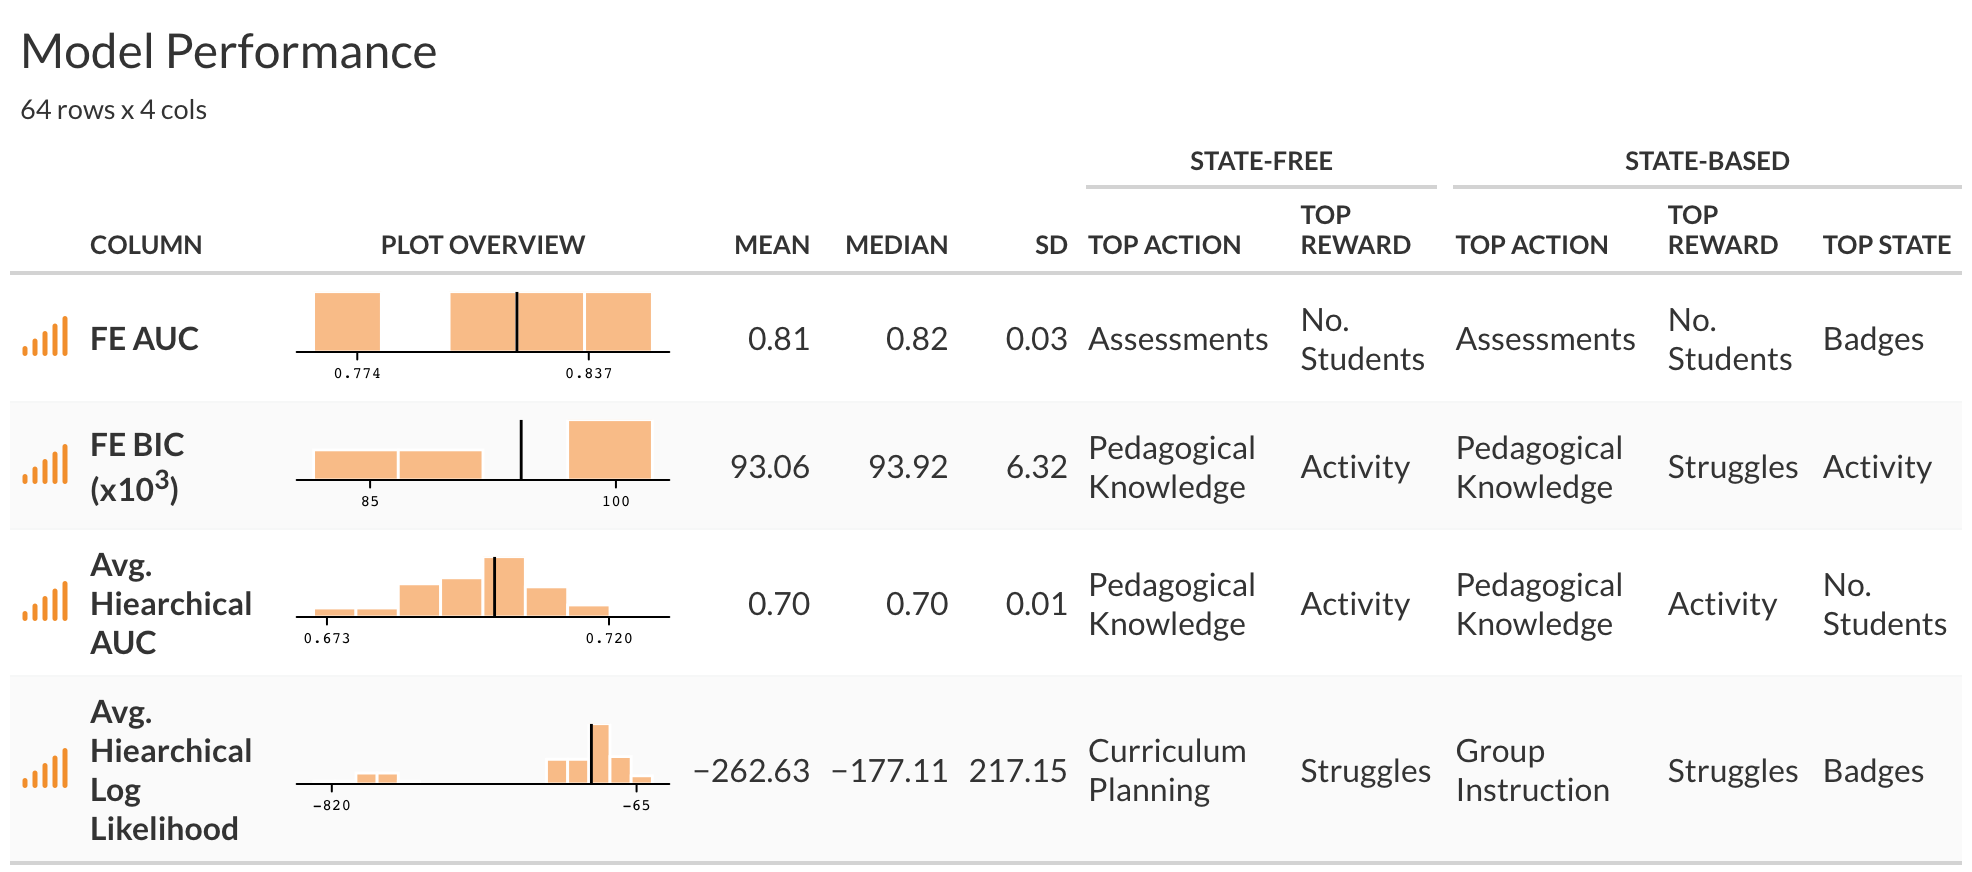
\includegraphics{images/tbl-RL-exploration.png}

}

\end{table}%

\paragraph{Model Performance}\label{model-performance}

Drawing on the resulting metrics, we strategically narrowed our focus to
the action-reward-state configurations that most closely align with
Reinforcement Learning (RL) principles. Figure~\ref{fig-RL-exploration}
delineates the top 25 models based on their high fixed-effects Area
Under the Curve (AUC) and mean teacher-specific AUC, as well as their
parsimonious Bayesian Information Criterion (BIC) and higher mean
teacher-specific log-likelihood.

Panel A of the figure highlights six state-free models. Each point on
the plot represents a different model, identified by its BIC and average
teacher-specific AUC. Within this framework, the actions of
``Activities'' and ``Assessments'' stand out, connected to rewards like
``Completion,'' ``No.~Sessions,'' and ``No.~Students.'' Panel B
spotlights 19 state-based models. In this plot, ``Scaffolding'' and
``Activities'' also emerge as the primary actions.

These visualizations highlight ``Scaffolding'' and ``Activities'' as
best-fit actions. However, the choice of associated rewards and states
is unclear, suggesting the need to fit RL models using all
configurations featuring these two actions.

\begin{figure}

\begin{minipage}{0.50\linewidth}

\centering{

\includegraphics{zearn_files/figure-pdf/fig-RL-exploration-1.pdf}

}

\subcaption{\label{fig-RL-exploration-1}State-free}

\end{minipage}%
%
\begin{minipage}{0.50\linewidth}

\centering{

\includegraphics{zearn_files/figure-pdf/fig-RL-exploration-2.pdf}

}

\subcaption{\label{fig-RL-exploration-2}State-dependent}

\end{minipage}%

\caption{\label{fig-RL-exploration}Selection of Actions, Rewards, and
States for Reinforcement Learning Analysis. The plots show the
performance metrics of logistic regression models designed to capture
characteristics similar to reinforcement learning models. The AUC and
BIC values are plotted separately for state-free and state-dependent
contexts. Models closest to the upper-left corners indicate a more
optimal balance between parsimony and accuracy in capturing RL-like
teacher behaviors.}

\end{figure}%

\paragraph{Model Interpretability}\label{model-interpretability}

Prior to fitting the reinforcement learning (RL) models, we analyzed the
regression coefficients in our best-fitting logit models to identify
patterns that align with RL principles. Our primary focus was on the
relationship between rewards and actions. Their interaction should
positively influence future actions for desired outcomes (e.g., lesson
completion) and negatively for undesired outcomes (e.g., struggles).
Additionally, we examined the effect of current states on strategic
action selection and the interaction between states and lagged actions
to indicate how actions attain and maintain desired states.

We re-estimated the models with scaled independent variables, allowing
for a direct coefficient comparison. In this context, a unit increase in
these variables equates to a one standard deviation increase.
Table~\ref{tbl-re-estimation-statefree} and
Table~\ref{tbl-re-estimation} summarize these results, presenting a
coherent overview of the standardized coefficients and highlighting the
significance of interactions between rewards, states, and lagged
actions.

The results convey that no singular approach fits all educational
contexts. Instead, a spectrum of pedagogical strategies exists, with
specific teaching methods aligning more closely with the principles of
RL. By focusing on coefficients that display RL-like effects,
particularly the interaction term R(t-1) x A(t-2), we identified
dominant strategies that include 1) Action: Group Instruction with
Reward: Struggles, and 2) Action: Group Instruction with Reward:
Activity and State: Badges.

In contrast, Figure~\ref{fig-RL-exploration} favors models that occupy
the upper-left quadrant, indicative of an optimized balance between
model complexity and predictive accuracy. Noteworthy configurations
include 1) Action: Pedagogical Knowledge with Reward: Activity, and 2)
Action: Pedagogical Knowledge with Reward: Activity, State: Number of
Students.

These configurations highlight teacher individual differences and
support the idea that using a hybrid modeling approach could improve the
process of fitting RL.

\newpage
\KOMAoptions{paper=landscape,pagesize}
\recalctypearea
{\areaset[current]{\dimexpr\textwidth\relax}{\textheight}
\setlength{\marginparwidth}{0pt}
\scriptsize

\begin{longtable}{l|l|rrrrrr}

\caption{\label{tbl-re-estimation-statefree}State-Free Mixed Effects
Logistic Regression Results}

\tabularnewline

\caption*{
{\large Summary of Model Coefficients}
} \\ 
\toprule
\multicolumn{2}{l}{} & \multicolumn{4}{c}{Group Instruction} & \multicolumn{2}{c}{Pedagogical Knowledge} \\ 
\cmidrule(lr){3-6} \cmidrule(lr){7-8}
\multicolumn{2}{l}{} & Activity & Badges & No. Students & Struggles & Activity & No. Students \\ 
\midrule\addlinespace[2.5pt]
R(t-1) x 
 A(t-1) & Mean & $-0.03$ & $1.59$ & $-0.72$ & $0.20$ & $-0.26$ & $-1.15$ \\ 
 & SD & $2.40$ & $21.96$ & $6.81$ & $3.27$ & $2.65$ & $6.36$ \\ 
 & Q1 & $-1.25$ & $-10.33$ & $-2.31$ & $-1.22$ & $-1.28$ & $-2.92$ \\ 
 & Median & $0.00$ & $0.43$ & $-0.37$ & $0.03$ & $-0.06$ & $-0.55$ \\ 
 & Q3 & $1.04$ & $10.03$ & $1.18$ & $1.51$ & $1.08$ & $1.02$ \\ 
 & RL-like & $49.09\%$ & $51.65\%$ & $42.71\%$ & $50.36\%$ & $47.09\%$ & $39.02\%$ \\ 
\midrule\addlinespace[2.5pt]
R(t-1) x 
 A(t-2) & Mean & $0.02$ & $-3.24$ & $0.65$ & $0.27$ & $-0.06$ & $-0.30$ \\ 
 & SD & $3.00$ & $26.98$ & $10.22$ & $3.59$ & $3.00$ & $9.98$ \\ 
 & Q1 & $-1.42$ & $-15.33$ & $-2.47$ & $-1.14$ & $-1.15$ & $-2.55$ \\ 
 & Median & $0.00$ & $-3.04$ & $0.02$ & $0.22$ & $0.04$ & $0.19$ \\ 
 & Q3 & $1.31$ & $7.11$ & $2.96$ & $1.86$ & $1.21$ & $3.31$ \\ 
 & RL-like & $49.77\%$ & $41.98\%$ & $50.38\%$ & $54.24\%$ & $50.79\%$ & $52.89\%$ \\ 
\midrule\addlinespace[2.5pt]
R(t-2) x 
 A(t-2) & Mean & $-0.11$ & $-0.05$ & $-0.39$ & $0.10$ & $-0.19$ & $-0.17$ \\ 
 & SD & $2.70$ & $22.30$ & $8.41$ & $3.83$ & $2.90$ & $10.15$ \\ 
 & Q1 & $-1.21$ & $-9.45$ & $-2.93$ & $-1.05$ & $-1.43$ & $-3.70$ \\ 
 & Median & $-0.13$ & $0.01$ & $-0.19$ & $0.20$ & $-0.11$ & $-0.53$ \\ 
 & Q3 & $1.10$ & $10.84$ & $2.80$ & $1.46$ & $0.86$ & $2.37$ \\ 
 & RL-like & $47.27\%$ & $50.33\%$ & $47.57\%$ & $53.27\%$ & $45.77\%$ & $42.49\%$ \\ 
\midrule\addlinespace[2.5pt]
N & — & $440.00$ & $455.00$ & $391.00$ & $413.00$ & $378.00$ & $346.00$ \\ 
\bottomrule

\end{longtable}

\newpage{}

\begin{longtable}{l|l|rrrrrrrrrrrrrrr}

\caption{\label{tbl-re-estimation}State-Based Mixed Effects Logistic
Regression Results}

\tabularnewline

\caption*{
{\large Summary of Model Coefficients}
} \\ 
\toprule
\multicolumn{2}{l}{} & \multicolumn{8}{c}{Group Instruction} & \multicolumn{7}{c}{Pedagogical Knowledge} \\ 
\cmidrule(lr){3-10} \cmidrule(lr){11-17}
\multicolumn{2}{l}{} & \multicolumn{2}{c}{Activity} & \multicolumn{2}{c}{Badges} & No. Students & \multicolumn{3}{c}{Struggles} & \multicolumn{3}{c}{Activity} & \multicolumn{2}{c}{No. Students} & \multicolumn{2}{c}{Struggles} \\ 
\cmidrule(lr){3-4} \cmidrule(lr){5-6} \cmidrule(lr){7-7} \cmidrule(lr){8-10} \cmidrule(lr){11-13} \cmidrule(lr){14-15} \cmidrule(lr){16-17}
\multicolumn{2}{l}{} & Badges & Struggles & Activity & No. Students & Badges & Activity & Badges & No. Students & Badges & No. Students & Struggles & Activity & Struggles & Activity & Badges \\ 
\midrule\addlinespace[2.5pt]
R(t-1) x 
 A(t-1) & Mean & $-0.11$ & $-0.13$ & $-0.38$ & $-0.21$ & $-0.75$ & $0.42$ & $0.20$ & $0.32$ & $-0.44$ & $-0.38$ & $-0.24$ & $-1.09$ & $-1.32$ & $0.72$ & $0.63$ \\ 
 & SD & $3.19$ & $3.69$ & $4.16$ & $3.48$ & $6.37$ & $4.22$ & $4.61$ & $4.58$ & $4.63$ & $5.13$ & $3.70$ & $9.56$ & $5.09$ & $6.11$ & $5.19$ \\ 
 & Q1 & $-1.52$ & $-1.45$ & $-1.78$ & $-1.70$ & $-2.43$ & $-1.23$ & $-1.42$ & $-1.44$ & $-1.58$ & $-1.48$ & $-1.86$ & $-3.31$ & $-3.02$ & $-1.26$ & $-1.38$ \\ 
 & Median & $-0.02$ & $0.01$ & $-0.10$ & $-0.06$ & $-0.22$ & $0.18$ & $0.07$ & $0.05$ & $-0.16$ & $-0.15$ & $-0.11$ & $-0.55$ & $-0.68$ & $0.27$ & $0.09$ \\ 
 & Q3 & $1.13$ & $1.27$ & $1.33$ & $1.22$ & $1.35$ & $2.02$ & $1.80$ & $1.83$ & $1.32$ & $1.23$ & $1.23$ & $1.54$ & $1.04$ & $2.02$ & $2.10$ \\ 
 & RL-like & $48.06\%$ & $50.36\%$ & $46.44\%$ & $47.72\%$ & $44.67\%$ & $53.02\%$ & $50.97\%$ & $50.90\%$ & $47.28\%$ & $45.65\%$ & $46.35\%$ & $41.30\%$ & $38.81\%$ & $54.79\%$ & $52.26\%$ \\ 
\midrule\addlinespace[2.5pt]
R(t-1) x 
 A(t-2) & Mean & $0.38$ & $-0.60$ & $-0.13$ & $0.26$ & $0.43$ & $0.68$ & $0.31$ & $-0.05$ & $0.08$ & $0.25$ & $-0.25$ & $0.09$ & $0.17$ & $-0.63$ & $-0.38$ \\ 
 & SD & $7.65$ & $9.95$ & $10.39$ & $10.49$ & $14.67$ & $12.45$ & $11.61$ & $5.66$ & $16.42$ & $14.01$ & $5.44$ & $26.15$ & $7.13$ & $13.43$ & $6.25$ \\ 
 & Q1 & $-1.58$ & $-1.99$ & $-2.63$ & $-2.09$ & $-3.92$ & $-1.46$ & $-1.22$ & $-1.65$ & $-2.19$ & $-1.36$ & $-1.79$ & $-4.20$ & $-3.58$ & $-2.40$ & $-2.24$ \\ 
 & Median & $0.46$ & $-0.08$ & $-0.25$ & $0.01$ & $0.00$ & $0.24$ & $0.21$ & $0.20$ & $0.08$ & $0.05$ & $0.01$ & $0.44$ & $0.00$ & $0.00$ & $0.00$ \\ 
 & Q3 & $2.46$ & $1.41$ & $2.04$ & $1.83$ & $3.68$ & $2.31$ & $2.38$ & $2.04$ & $2.34$ & $1.73$ & $1.54$ & $4.86$ & $3.61$ & $2.27$ & $1.84$ \\ 
 & RL-like & $57.52\%$ & $48.69\%$ & $45.95\%$ & $50.25\%$ & $49.13\%$ & $53.77\%$ & $54.85\%$ & $52.69\%$ & $50.54\%$ & $51.09\%$ & $50.52\%$ & $52.72\%$ & $49.25\%$ & $49.59\%$ & $49.15\%$ \\ 
\midrule\addlinespace[2.5pt]
R(t-2) x 
 A(t-2) & Mean & $-0.36$ & $-0.34$ & $0.25$ & $0.25$ & $-0.48$ & $-0.07$ & $0.00$ & $0.20$ & $-0.35$ & $0.03$ & $-0.22$ & $-0.35$ & $-0.83$ & $-1.14$ & $0.31$ \\ 
 & SD & $6.59$ & $9.45$ & $8.99$ & $7.10$ & $14.68$ & $9.75$ & $12.59$ & $7.14$ & $10.99$ & $10.12$ & $4.76$ & $33.27$ & $6.69$ & $13.59$ & $6.35$ \\ 
 & Q1 & $-1.65$ & $-1.31$ & $-1.63$ & $-1.54$ & $-3.94$ & $-1.24$ & $-1.47$ & $-1.31$ & $-1.80$ & $-1.58$ & $-1.76$ & $-4.82$ & $-3.72$ & $-2.31$ & $-1.59$ \\ 
 & Median & $-0.24$ & $-0.09$ & $0.02$ & $0.21$ & $-0.17$ & $0.18$ & $0.16$ & $0.34$ & $-0.19$ & $-0.01$ & $-0.17$ & $-0.62$ & $-0.33$ & $-0.28$ & $0.00$ \\ 
 & Q3 & $1.11$ & $1.23$ & $1.74$ & $1.71$ & $3.38$ & $1.92$ & $1.87$ & $1.98$ & $1.28$ & $1.53$ & $1.10$ & $3.16$ & $2.10$ & $1.76$ & $1.63$ \\ 
 & RL-like & $43.20\%$ & $47.26\%$ & $50.12\%$ & $53.55\%$ & $47.64\%$ & $53.77\%$ & $53.16\%$ & $55.75\%$ & $45.11\%$ & $48.37\%$ & $43.23\%$ & $43.21\%$ & $43.88\%$ & $46.03\%$ & $49.44\%$ \\ 
\midrule\addlinespace[2.5pt]
S(t) & Mean & $0.09$ & $-0.21$ & $-0.09$ & $0.75$ & $-0.23$ & $-0.01$ & $0.00$ & $0.44$ & $0.37$ & $0.93$ & $0.03$ & $-0.18$ & $-0.19$ & $-0.08$ & $0.07$ \\ 
 & SD & $2.72$ & $2.31$ & $2.40$ & $2.60$ & $1.87$ & $1.45$ & $1.63$ & $2.39$ & $2.51$ & $2.94$ & $1.89$ & $1.59$ & $1.54$ & $1.21$ & $1.55$ \\ 
 & Q1 & $-1.11$ & $-0.96$ & $-1.19$ & $-0.68$ & $-1.09$ & $-0.61$ & $-0.75$ & $-0.50$ & $-0.92$ & $-0.54$ & $-0.94$ & $-0.87$ & $-0.99$ & $-0.63$ & $-0.57$ \\ 
 & Median & $0.13$ & $-0.03$ & $0.06$ & $0.33$ & $-0.05$ & $-0.04$ & $0.00$ & $0.19$ & $0.13$ & $0.40$ & $0.03$ & $-0.05$ & $-0.06$ & $-0.07$ & $-0.03$ \\ 
 & Q3 & $1.23$ & $0.73$ & $0.96$ & $1.74$ & $0.77$ & $0.77$ & $0.86$ & $1.32$ & $1.62$ & $1.52$ & $0.80$ & $0.65$ & $0.59$ & $0.51$ & $0.72$ \\ 
 & RL-like & $52.18\%$ & $48.69\%$ & $50.86\%$ & $59.39\%$ & $48.39\%$ & $47.99\%$ & $50.00\%$ & $56.78\%$ & $52.99\%$ & $58.97\%$ & $51.04\%$ & $48.37\%$ & $47.16\%$ & $47.67\%$ & $48.59\%$ \\ 
\midrule\addlinespace[2.5pt]
S(t) x 
 A(t-1) & Mean & $-0.78$ & $0.38$ & $0.13$ & $-0.98$ & $0.02$ & $-0.68$ & $-0.93$ & $-0.27$ & $-1.43$ & $-0.96$ & $0.04$ & $-0.11$ & $0.46$ & $-1.01$ & $-0.68$ \\ 
 & SD & $7.71$ & $10.07$ & $7.57$ & $11.39$ & $6.35$ & $9.65$ & $10.26$ & $8.66$ & $16.86$ & $13.25$ & $6.75$ & $11.33$ & $4.32$ & $9.27$ & $5.09$ \\ 
 & Q1 & $-2.74$ & $-1.27$ & $-1.83$ & $-3.06$ & $-1.69$ & $-1.53$ & $-1.85$ & $-2.10$ & $-2.97$ & $-4.27$ & $-2.12$ & $-1.55$ & $-1.11$ & $-1.72$ & $-2.26$ \\ 
 & Median & $-0.31$ & $0.31$ & $0.06$ & $-0.20$ & $-0.01$ & $-0.03$ & $-0.14$ & $-0.06$ & $-0.12$ & $-0.14$ & $0.02$ & $0.05$ & $0.12$ & $0.00$ & $-0.22$ \\ 
 & Q3 & $1.82$ & $2.25$ & $2.03$ & $1.83$ & $1.89$ & $1.05$ & $1.31$ & $1.84$ & $2.06$ & $2.12$ & $2.01$ & $1.49$ & $1.63$ & $1.52$ & $1.41$ \\ 
 & RL-like & $46.60\%$ & $57.28\%$ & $50.61\%$ & $46.45\%$ & $48.88\%$ & $48.99\%$ & $46.12\%$ & $48.59\%$ & $47.01\%$ & $46.47\%$ & $50.26\%$ & $51.90\%$ & $52.54\%$ & $50.14\%$ & $45.48\%$ \\ 
\midrule\addlinespace[2.5pt]
N & — & $412.00$ & $419.00$ & $407.00$ & $394.00$ & $403.00$ & $398.00$ & $412.00$ & $391.00$ & $368.00$ & $368.00$ & $384.00$ & $368.00$ & $335.00$ & $365.00$ & $354.00$ \\ 
\bottomrule

\end{longtable}

}
\newpage
\KOMAoptions{paper=portrait,pagesize}
\recalctypearea

\subsection{Estimating RL Models}\label{estimating-rl-models}

This section aims to identify and evaluate reinforcement learning (RL)
models that best represent the teaching strategies derived from our
data. The performance of each model is quantified by computing the log
evidence, a metric that balances model fit against complexity, similar
to the Bayesian Information Criterion. This metric is critical as it
provides a common ground for comparing models with varying degrees of
freedom, ensuring that our selection process favors models that capture
the essential patterns without overfitting. Our first step will be to
choose the most suitable model based on this performance score. Then, we
will carefully analyze it for any discernible patterns that may help us
understand the teaching strategies present in our dataset.

\paragraph{Distribution of Model
Performance}\label{distribution-of-model-performance}

After estimating Q-learning and Actor-Critic Models for all potential
action-reward-state configurations, specifically focusing on the actions
``Pedagogical Knowledge'' and ``Group Instruction,'' we plotted their
log evidence scores in Figure~\ref{fig-log-evidence-histogram}. The
resulting histogram illustrates the variability in model fit for both
Q-learning and Actor-Critic RL models. The diversity in log evidence
scores highlights the distinct behaviors of each model. At the same
time, the bimodal distribution suggests that the two action variables
can yield significantly different model fits, as we saw in our logistic
regression models.

\begin{figure}

\centering{

\includegraphics{zearn_files/figure-pdf/fig-log-evidence-histogram-1.pdf}

}

\caption{\label{fig-log-evidence-histogram}Histogram of Log Evidences
for Q-learning and Actor-Critic Models. The graph illustrates the
distribution of models based on their log evidence (i.e., penalized
likelihood) across Actor-Critic and Q-learning models.}

\end{figure}%

\paragraph{Standout Models}\label{standout-models}

Our computational analysis identified a distinct group of models that
excelled in their high log evidence scores. Interestingly, all
top-performing models featured ``Pedagogical Knowledge'' as their
primary action. Table~\ref{tbl-top-CBM} provides a breakdown of scores
for different combinations of rewards and states under this action,
offering insight into the comparative performance of various model
setups. Notably, models with ``Badges'' and ``Activity'' as their
rewards outperform others, as do state-free models, likely due to their
higher simplicity.

\begin{longtable}{l|lr}

\caption{\label{tbl-top-CBM}Best-fit models. The table lists the models
with the highest log evidence scores by their rewards, states. All
models are based on the action `Pedagogical Knowledge.'}

\tabularnewline

\toprule
\multicolumn{1}{l}{Reward} & State & Log Evidence \\ 
\midrule\addlinespace[2.5pt]
Badges & Struggles, No. Students & $-2,411.5$ \\ 
 & — & $-4,386.8$ \\ 
 & No. Students & $-4,792.6$ \\ 
 & Struggles, No. Students, Activity & $-4,858.0$ \\ 
\midrule\addlinespace[2.5pt]
Activity & — & $-4,381.0$ \\ 
 & Badges & $-4,855.0$ \\ 
 & Struggles No. Students & $-4,862.5$ \\ 
 & Badges, Struggles, No. Students & $-4,882.2$ \\ 
\midrule\addlinespace[2.5pt]
No. Students & — & $-4,381.2$ \\ 
 & Badges, Struggles & $-4,875.1$ \\ 
\midrule\addlinespace[2.5pt]
Struggles & — & $-4,410.1$ \\ 
 & Badges, No. Students, Activity & $-4,881.5$ \\ 
 & No. Students, Activity & $-4,983.6$ \\ 
 & Activity & $-5,017.6$ \\ 
\bottomrule

\end{longtable}

\paragraph{Hierarchical Bayesian Inference (HBI) Results and Model
Comparison}\label{hierarchical-bayesian-inference-hbi-results-and-model-comparison}

To further refine our selection, we employ Hierarchical Bayesian
Inference (HBI) to perform a more detailed comparison of the selected
models. This statistical approach allows us to compare models not just
by their individual fits, but also by their ability to explain data
across different subjects. In interpreting the results from HBI, we
observed the differential performances of Q-learning (QL) and
Actor-Critic (AC) models. Table~\ref{tbl-CBM-HBI} provides quantifiable
insights into how frequently each model emerged as the best fit across
iterations (Model Frequency) and the sum log likelihood across subjects
(Log Likelihood). Notably, we see that in both model types, models that
used Badges and Activity as their rewards overperformed. The HBI results
and corresponding model comparison statistics serve as our basis for
selecting the most appropriate RL model.

\begin{longtable}{l|rrrr}

\caption{\label{tbl-CBM-HBI}Top Q-learning and Actor-Critic models. The
tables quantify performance under hierarchical bayesian inference
through model frequencies and the sum of log likelihoods. All models are
based on the action `Pedagogical Knowledge.'}

\tabularnewline

\toprule
\multicolumn{1}{l}{} & \multicolumn{4}{c}{Pedagogical Knowledge} \\ 
\cmidrule(lr){2-5}
\multicolumn{1}{l}{} & Badges & Struggles & No. Students & Activity \\ 
\midrule\addlinespace[2.5pt]
Model Frequency & $60.5\%$ & $0.0\%$ & $39.5\%$ & $0.0\%$ \\ 
\midrule\addlinespace[2.5pt]
Log Likelihood & $-4,362.7$ & $-3,454.1$ & $-4,830.9$ & $-3,500.2$ \\ 
\bottomrule

\end{longtable}

\begin{longtable}{l|rrrrr}

\caption{\label{tbl-CBM-HBI}Top Q-learning and Actor-Critic models. The
tables quantify performance under hierarchical bayesian inference
through model frequencies and the sum of log likelihoods. All models are
based on the action `Pedagogical Knowledge.'}

\tabularnewline

\toprule
\multicolumn{1}{l}{} & \multicolumn{5}{c}{Pedagogical Knowledge} \\ 
\cmidrule(lr){2-6}
\multicolumn{1}{l}{} & \multicolumn{2}{c}{Badges} & No. Students & \multicolumn{2}{c}{Activity} \\ 
\cmidrule(lr){2-3} \cmidrule(lr){4-4} \cmidrule(lr){5-6}
\multicolumn{1}{l}{} & No. Students & Struggles, No. Students, Activity & Badges, Struggles & Badges & Struggles, No. Students \\ 
\midrule\addlinespace[2.5pt]
Model Frequency & $80.5\%$ & $0.0\%$ & $0.0\%$ & $19.5\%$ & $0.0\%$ \\ 
\midrule\addlinespace[2.5pt]
Log Likelihood & $35,289.0$ & $-1,862.6$ & $-1,886.3$ & $-3,812.7$ & $-1,872.9$ \\ 
\bottomrule

\end{longtable}

\paragraph{Hybrid Models Comparison}\label{hybrid-models-comparison}

In pursuit of a more comprehensive understanding of our model space, we
turn to the investigation of hybrid models that blend elements from both
the Logit and RL frameworks. These hybrids offer a potentially more
nuanced approach to representing the complexities of learning behavior,
aiming to combine the strengths of logistic regression with the dynamic
adaptability inherent in reinforcement learning techniques.

The comparative analysis of these models is conducted via Hierarchical
Bayesian Inference. Table~\ref{tbl-CBM-second} shows the performance for
different reward and state contexts across the logit model, the
corresponding reinforcement learning model (Q-learning model in
state-free cases and Actor-Critic in state-based cases), and two hybrid
configurations (i.e., Logit and RL hybrids, Q-learning and Actor-Critic
hybrids). Our evaluation suggests that any potential performance gain
from hybridizing do not outweigh the cost of increased model complexity.

\setlength{\LTpost}{0mm}

\begin{longtable}{l|lrrrr}

\caption{\label{tbl-CBM-second}Comparative fit of hybrid models. The
table presents the proportion of data that is best explained by each
model configuration, including hybrid models. All models are based on
the action `Pedagogical Knowledge.'}

\tabularnewline

\toprule
\multicolumn{1}{l}{Reward} & State & Logit & RL\textsuperscript{\textit{1}} & Logit-RL Hybrid\textsuperscript{\textit{2}} & QL-AC Hybrid\textsuperscript{\textit{3}} \\ 
\midrule\addlinespace[2.5pt]
Activity & — & $90.6\%$ & $9.4\%$ & $0.0\%$ & $0.0\%$ \\ 
 & Struggles, No. Students & $24.4\%$ & $75.6\%$ & $0.0\%$ & $0.0\%$ \\ 
\midrule\addlinespace[2.5pt]
Badges & — & $90.9\%$ & $9.1\%$ & $0.0\%$ & $0.0\%$ \\ 
 & No. Students & $31.0\%$ & $69.0\%$ & $0.0\%$ & $0.0\%$ \\ 
\bottomrule

\end{longtable}

\begin{minipage}{\linewidth}
\textsuperscript{\textit{1}}Q-learning model in state-free case and Actor-Critic in state-based case.\\
\textsuperscript{\textit{2}}Combines predictions of Logit and RL models.\\
\textsuperscript{\textit{3}}Combines predictions of Q-learning (state-free) and Actor-Critic (state-based) models.\\
\end{minipage}

\paragraph{Top Model Selection}\label{top-model-selection-1}

In the final stages of our model selection process, we converge on the
identification of the top-performing models. By assessing the frequency
with which each model provides the best explanation for the observed
data, we make an informed decisions about their suitability for
capturing teacher behavioral patterns. Table~\ref{tbl-CBM-final}
distills these results by juxtaposing the models based on the rewards
`Activity' and `Badges.' The table reveals that the `Badges'
consistently outperforms `Activity' across logit and actor-critic
models, indicating its superior explanatory power in the context of
pedagogical knowledge.

\begin{longtable}{l|rrrr}

\caption{\label{tbl-CBM-final}Top Model Comparison. The table compares
the leading models on their ability to explain the data, as indicated by
the model frequencies. All models are based on the action `Pedagogical
Knowledge.'}

\tabularnewline

\toprule
\multicolumn{1}{l}{} & \multicolumn{4}{c}{Pedagogical Knowledge} \\ 
\cmidrule(lr){2-5}
\multicolumn{1}{l}{} & \multicolumn{2}{c}{Activity} & \multicolumn{2}{c}{Badges} \\ 
\cmidrule(lr){2-3} \cmidrule(lr){4-5}
\multicolumn{1}{l}{} & None & Struggles, No. Students & None & No. Students \\ 
\midrule\addlinespace[2.5pt]
Model Frequency & $0.0\%$ & $0.0\%$ & $21.4\%$ & $78.6\%$ \\ 
\bottomrule

\end{longtable}

\subsection{Heterogeneity Analyses}\label{heterogeneity-analyses}

In our investigation of different pedagogical strategies in Zearn, we
analyzed the impact of teacher characteristics on the success of
reinforcement learning (RL) models.

The histogram of teacher-specific log-likelihoods in
Figure~\ref{fig-loglik-histogram} reveals a centralized distribution,
indicating consistency in model performance across teachers. Most
teachers' data aligned with the model around the median log-likelihood,
suggesting a typical teaching strategy efficacy pattern. This central
tendency indicates the model's reliability in capturing the underlying
decision-making processes. However, the spread of the histogram also
implies variations, highlighting the diversity in teaching strategies,
which warrants further investigation into individual differences.

\begin{figure}

\centering{

\includegraphics{zearn_files/figure-pdf/fig-loglik-histogram-1.pdf}

}

\caption{\label{fig-loglik-histogram}Histogram of teacher-specific log
likelihood}

\end{figure}%

In addition, we analyzed teacher-specific parameters to capture these
individual differences. Figure~\ref{fig-params-histogram} provides a set
of violin plots depicting a range of teacher behaviors and tendencies.
We observed a wide range of learning rates, indicating differences in
how quickly teachers adjusted their teaching based on student
interactions. The distribution of the temperature parameter indicated
varying levels of strategic consistency. Initial policy parameters are
very close to zero, implying a ``blank slate'' for educators before
making adjustments. Finally, the range in cost parameters pointed to a
subjective assessment of resource investment in different teaching
actions, revealing differences in perceived effort or resources required
for specific teaching approaches.

\begin{figure}

\begin{minipage}{0.33\linewidth}

\centering{

\includegraphics{zearn_files/figure-pdf/fig-params-histogram-1.pdf}

}

\subcaption{\label{fig-params-histogram-1}Value weights learning rate}

\end{minipage}%
%
\begin{minipage}{0.33\linewidth}

\centering{

\includegraphics{zearn_files/figure-pdf/fig-params-histogram-2.pdf}

}

\subcaption{\label{fig-params-histogram-2}Policy weights learning rate}

\end{minipage}%
%
\begin{minipage}{0.33\linewidth}

\centering{

\includegraphics{zearn_files/figure-pdf/fig-params-histogram-3.pdf}

}

\subcaption{\label{fig-params-histogram-3}Discount factor}

\end{minipage}%
\newline
\begin{minipage}{0.33\linewidth}

\centering{

\includegraphics{zearn_files/figure-pdf/fig-params-histogram-4.pdf}

}

\subcaption{\label{fig-params-histogram-4}Temperature}

\end{minipage}%
%
\begin{minipage}{0.33\linewidth}

\centering{

\includegraphics{zearn_files/figure-pdf/fig-params-histogram-5.pdf}

}

\subcaption{\label{fig-params-histogram-5}Initial policy}

\end{minipage}%
%
\begin{minipage}{0.33\linewidth}

\centering{

\includegraphics{zearn_files/figure-pdf/fig-params-histogram-6.pdf}

}

\subcaption{\label{fig-params-histogram-6}Initial value}

\end{minipage}%
\newline
\begin{minipage}{0.33\linewidth}

\centering{

\includegraphics{zearn_files/figure-pdf/fig-params-histogram-7.pdf}

}

\subcaption{\label{fig-params-histogram-7}Cost}

\end{minipage}%

\caption{\label{fig-params-histogram}Histogram of Teacher-Specific
Parameters}

\end{figure}%

Our heterogeneity analysis also included comparing teachers classified
into Logit or Actor-Critic models. Table~\ref{tbl-CBM-teachers} displays
these results; however, no differences were statistically significant
after p-value correction.

\begin{longtable}[]{@{}
  >{\raggedright\arraybackslash}p{(\columnwidth - 12\tabcolsep) * \real{0.1667}}
  >{\centering\arraybackslash}p{(\columnwidth - 12\tabcolsep) * \real{0.0614}}
  >{\centering\arraybackslash}p{(\columnwidth - 12\tabcolsep) * \real{0.1667}}
  >{\centering\arraybackslash}p{(\columnwidth - 12\tabcolsep) * \real{0.2368}}
  >{\centering\arraybackslash}p{(\columnwidth - 12\tabcolsep) * \real{0.1404}}
  >{\centering\arraybackslash}p{(\columnwidth - 12\tabcolsep) * \real{0.1140}}
  >{\centering\arraybackslash}p{(\columnwidth - 12\tabcolsep) * \real{0.1140}}@{}}

\caption{\label{tbl-CBM-teachers}Comparison of Teacher Characteristics
by Model Type. The table presents the differences in means across
various characteristics between teachers classified into Logit or
Actor-Critic models.}

\tabularnewline

\toprule\noalign{}
\begin{minipage}[b]{\linewidth}\raggedright
\textbf{Characteristic}
\end{minipage} & \begin{minipage}[b]{\linewidth}\centering
\textbf{N}
\end{minipage} & \begin{minipage}[b]{\linewidth}\centering
\textbf{Logit}, N = 68
\end{minipage} & \begin{minipage}[b]{\linewidth}\centering
\textbf{Actor-Critic}, N = 227
\end{minipage} & \begin{minipage}[b]{\linewidth}\centering
\textbf{Difference}
\end{minipage} & \begin{minipage}[b]{\linewidth}\centering
\textbf{p-value}
\end{minipage} & \begin{minipage}[b]{\linewidth}\centering
\textbf{q-value}
\end{minipage} \\
\midrule\noalign{}
\endhead
\bottomrule\noalign{}
\endlastfoot
Charter School & 295 & 2.9\% & 8.4\% & -5.4\% & 0.2 & 0.3 \\
Paid Account & 295 & 76\% & 76\% & 0.70\% & \textgreater0.9 &
\textgreater0.9 \\
Poverty & 273 & & & 0.47 & & \\
0-40\% (Low) & & 28\% & 26\% & & & \\
40-75\% (Mid-High) & & 66\% & 52\% & & & \\
75\%+ (High) & & 6.2\% & 22\% & & & \\
No.~of Weeks & 295 & 28 (7) & 27 (8) & 1.1 & 0.3 & 0.4 \\
Active Students & 295 & 70 (31) & 60 (33) & 9.5 & 0.030 & 0.14 \\
Avg. Badges & 295 & 46 (20) & 41 (22) & 4.9 & 0.081 & 0.15 \\
Avg. Tower Alerts & 295 & 25 (15) & 25 (17) & 0.44 & 0.8 &
\textgreater0.9 \\
Action & 295 & 0.56 (0.75) & 0.78 (0.92) & -0.22 & 0.052 & 0.15 \\
Reward & 295 & 2.07 (0.89) & 1.84 (0.99) & 0.23 & 0.074 & 0.15 \\
State & 295 & 2.00 (0.89) & 1.73 (0.93) & 0.27 & 0.029 & 0.14 \\

\end{longtable}

Additionally, we further differentiated teacher behaviors by splitting
the data based on log-likelihood, creating `Good Fit' and `Bad Fit'
model groups. Table~\ref{tbl-CBM-teachers-full} shows the differences
between these two groups, and the results indicate overall higher weekly
usage for teachers in the Good Fit group. With the exception of the
average number of tower alerts (i.e., corrected for number of weeks),
teachers in the Good Fit group had higher values across all variables,
suggesting a more engaged and effective teaching approach.

\begin{longtable}[]{@{}
  >{\raggedright\arraybackslash}p{(\columnwidth - 12\tabcolsep) * \real{0.1624}}
  >{\centering\arraybackslash}p{(\columnwidth - 12\tabcolsep) * \real{0.0598}}
  >{\centering\arraybackslash}p{(\columnwidth - 12\tabcolsep) * \real{0.2137}}
  >{\centering\arraybackslash}p{(\columnwidth - 12\tabcolsep) * \real{0.2051}}
  >{\centering\arraybackslash}p{(\columnwidth - 12\tabcolsep) * \real{0.1368}}
  >{\centering\arraybackslash}p{(\columnwidth - 12\tabcolsep) * \real{0.1111}}
  >{\centering\arraybackslash}p{(\columnwidth - 12\tabcolsep) * \real{0.1111}}@{}}

\caption{\label{tbl-CBM-teachers-full}Comparison of Teacher
Characteristics by Model Fit. The table presents the differences in
means across various characteristics between teachers classified into
Good Fit or Bad Fit groups.}

\tabularnewline

\toprule\noalign{}
\begin{minipage}[b]{\linewidth}\raggedright
\textbf{Characteristic}
\end{minipage} & \begin{minipage}[b]{\linewidth}\centering
\textbf{N}
\end{minipage} & \begin{minipage}[b]{\linewidth}\centering
\textbf{Good Fit}, N = 1,515
\end{minipage} & \begin{minipage}[b]{\linewidth}\centering
\textbf{Bad Fit}, N = 1,514
\end{minipage} & \begin{minipage}[b]{\linewidth}\centering
\textbf{Difference}
\end{minipage} & \begin{minipage}[b]{\linewidth}\centering
\textbf{p-value}
\end{minipage} & \begin{minipage}[b]{\linewidth}\centering
\textbf{q-value}
\end{minipage} \\
\midrule\noalign{}
\endhead
\bottomrule\noalign{}
\endlastfoot
Charter School & 3,029 & 8.3\% & 5.2\% & 3.0\% & 0.001 & 0.001 \\
Paid Zearn Account & 3,029 & 72\% & 86\% & -14\% & \textless0.001 &
\textless0.001 \\
Poverty & 2,834 & & & 0.15 & & \\
0-40\% (Low) & & 21\% & 24\% & & & \\
40-75\% (Mid-High) & & 54\% & 58\% & & & \\
75\%+ (High) & & 25\% & 19\% & & & \\
No.~of Weeks & 3,029 & 23 (9) & 31 (5) & -8.1 & \textless0.001 &
\textless0.001 \\
Active Students & 3,029 & 1.92 (0.80) & 2.29 (0.79) & -0.37 &
\textless0.001 & \textless0.001 \\
Avg. Badges & 3,029 & 1.25 (0.54) & 1.61 (0.53) & -0.36 & \textless0.001
& \textless0.001 \\
Avg. Tower Alerts & 3,029 & 0.86 (0.56) & 0.88 (0.49) & -0.02 & 0.3 &
0.3 \\
Action & 3,029 & 0.017 (0.026) & 0.031 (0.030) & -0.01 & \textless0.001
& \textless0.001 \\
Reward & 3,029 & 0.055 (0.024) & 0.072 (0.024) & -0.02 & \textless0.001
& \textless0.001 \\
State & 3,029 & 0.055 (0.023) & 0.065 (0.023) & -0.01 & \textless0.001 &
\textless0.001 \\

\end{longtable}

\subsection{Optimality}\label{optimality}

To understand what makes a teacher effective in helping students
complete their lessons, we carefully examined teachers' performance
across various parameters from the previous hierarchical model. We were
especially interested in the learning rate (``Alpha'') and the inverse
temperature (``Tau'') because of their potential impact on behavior
adaptation and decision consistency. We found that these parameters
correlated to the number of weekly badges earned by the average student
(i.e., average lesson completion) and Tower Alerts (i.e., students
struggling with the material).

Table~\ref{tbl-optimality} presents the coefficients of six different
linear regression models. Each model predicts the average weekly badges
earned per teacher (Models 1-3) or the average weekly Tower Alerts
(Models 4-6) based on different combinations of the parameters and
control variables. The control variables include the number of active
students, the number of classes taught by the teacher, the grade level,
the number of weeks, the poverty level, the income level, whether the
school is a charter school, and whether the school has a paid account.

These models revealed that the RL parameters do not significantly affect
tower alerts, as already suggested in Table~\ref{tbl-CBM-teachers-full}.
However, they correlate with badges: a higher learning rate for value
weights and initial value weights were linked to higher badges. A
positive correlation was also present for the estimated cost parameter.
On the other hand, a higher temperature parameter, discount rate, and
initial policy weights were negatively associated with badges.

\begin{table}

\caption{\label{tbl-optimality}Impact of RL parameters on Weekly Badges
and Tower Alerts. Six linear regression models were used to examine the
correlations between a teacher's RL parameters and two measures of
student engagement: average weekly Badges earned per student (Models
1-3) and average weekly Tower Alerts per student (Models 4-6). Models
2-3 and 5-6 also control for other variables including number of active
students, number of classes taught, grade level, weeks, poverty level,
income level, whether the school is a charter school, and whether the
school has a paid account. Coefficients and standard errors are provided
for each parameter in each model.}

\centering{

[!htbp] \centering 
  \caption{} 
  \label{} 
\begin{tabular}{@{\extracolsep{5pt}}lD{.}{.}{-3} D{.}{.}{-3} D{.}{.}{-3} D{.}{.}{-3} D{.}{.}{-3} D{.}{.}{-3} } 
\\[-1.8ex]\hline 
\hline \\[-1.8ex] 
 & \multicolumn{6}{c}{\textit{Dependent variable:}} \\ 
\cline{2-7} 
\\[-1.8ex] & \multicolumn{3}{c}{Badges} & \multicolumn{3}{c}{Tower Alerts} \\ 
\\[-1.8ex] & \multicolumn{1}{c}{(1)} & \multicolumn{1}{c}{(2)} & \multicolumn{1}{c}{(3)} & \multicolumn{1}{c}{(4)} & \multicolumn{1}{c}{(5)} & \multicolumn{1}{c}{(6)}\\ 
\hline \\[-1.8ex] 
 $\alpha_w$ & 0.241^{**} & 0.156^{*} & 0.137^{*} & -0.027 & -0.093 & -0.071 \\ 
  & (0.078) & (0.067) & (0.068) & (0.080) & (0.078) & (0.079) \\ 
  & & & & & & \\ 
 $\alpha_\theta$ & 0.131 & 0.068 & 0.067 & -0.001 & 0.008 & -0.068 \\ 
  & (0.068) & (0.058) & (0.058) & (0.069) & (0.067) & (0.068) \\ 
  & & & & & & \\ 
 $\gamma$ & -0.090^{*} & -0.078^{*} & -0.074^{*} & -0.022 & -0.027 & -0.045 \\ 
  & (0.037) & (0.031) & (0.032) & (0.037) & (0.036) & (0.037) \\ 
  & & & & & & \\ 
 $\tau$ & -0.372^{***} & -0.303^{***} & -0.161^{*} & 0.053 & 0.064 & 0.115 \\ 
  & (0.092) & (0.078) & (0.079) & (0.093) & (0.091) & (0.091) \\ 
  & & & & & & \\ 
 Cost & 0.559^{***} & 0.440^{***} & 0.428^{***} & 0.045 & 0.022 & 0.031 \\ 
  & (0.053) & (0.045) & (0.045) & (0.054) & (0.052) & (0.052) \\ 
  & & & & & & \\ 
 $\theta_{init}$ & -18.585^{***} & -11.072^{***} & -8.627^{***} & -5.249^{***} & -2.557 & -2.487 \\ 
  & (1.539) & (1.321) & (1.327) & (1.564) & (1.540) & (1.542) \\ 
  & & & & & & \\ 
 $w_{init}$ & 1.500^{***} & 0.943^{***} & 0.846^{***} & 0.174 & 0.001 & 0.077 \\ 
  & (0.113) & (0.097) & (0.096) & (0.114) & (0.113) & (0.112) \\ 
  & & & & & & \\ 
 No. of Active Students &  & 0.331^{***} & 0.294^{***} &  & 0.144^{***} & 0.097^{***} \\ 
  &  & (0.010) & (0.011) &  & (0.012) & (0.013) \\ 
  & & & & & & \\ 
 No. of Classes &  & -0.061^{***} & -0.044^{***} &  & 0.074^{***} & 0.013 \\ 
  &  & (0.009) & (0.010) &  & (0.010) & (0.012) \\ 
  & & & & & & \\ 
 Grade &  &  & 0.014^{***} &  &  & 0.001 \\ 
  &  &  & (0.001) &  &  & (0.001) \\ 
  & & & & & & \\ 
 No. of Weeks &  &  & 0.027 &  &  & 0.028 \\ 
  &  &  & (0.035) &  &  & (0.041) \\ 
  & & & & & & \\ 
 Poverty Level &  &  & 0.032 &  &  & 0.156^{***} \\ 
  &  &  & (0.021) &  &  & (0.025) \\ 
  & & & & & & \\ 
 Charter School & 5.379^{***} & 3.867^{***} & 3.657^{***} & 0.708 & 0.177 & -1.146 \\ 
  & (0.699) & (0.593) & (0.602) & (0.710) & (0.691) & (0.700) \\ 
  & & & & & & \\ 
\hline \\[-1.8ex] 
Control for Grade Level &  & Yes & Yes &  & Yes & Yes \\ 
Control for Poverty Level &  &  & Yes &  &  & Yes \\ 
Observations & \multicolumn{1}{c}{3,029} & \multicolumn{1}{c}{3,029} & \multicolumn{1}{c}{2,834} & \multicolumn{1}{c}{3,029} & \multicolumn{1}{c}{3,029} & \multicolumn{1}{c}{2,834} \\ 
R$^{2}$ & \multicolumn{1}{c}{0.143} & \multicolumn{1}{c}{0.386} & \multicolumn{1}{c}{0.455} & \multicolumn{1}{c}{0.004} & \multicolumn{1}{c}{0.061} & \multicolumn{1}{c}{0.158} \\ 
Adjusted R$^{2}$ & \multicolumn{1}{c}{0.141} & \multicolumn{1}{c}{0.384} & \multicolumn{1}{c}{0.452} & \multicolumn{1}{c}{0.002} & \multicolumn{1}{c}{0.058} & \multicolumn{1}{c}{0.152} \\ 
Residual Std. Error & \multicolumn{1}{c}{0.520 (df = 3021)} & \multicolumn{1}{c}{0.440 (df = 3019)} & \multicolumn{1}{c}{0.419 (df = 2814)} & \multicolumn{1}{c}{0.528 (df = 3021)} & \multicolumn{1}{c}{0.513 (df = 3019)} & \multicolumn{1}{c}{0.487 (df = 2814)} \\ 
F Statistic & \multicolumn{1}{c}{71.906$^{***}$ (df = 7; 3021)} & \multicolumn{1}{c}{211.033$^{***}$ (df = 9; 3019)} & \multicolumn{1}{c}{123.755$^{***}$ (df = 19; 2814)} & \multicolumn{1}{c}{1.922 (df = 7; 3021)} & \multicolumn{1}{c}{21.886$^{***}$ (df = 9; 3019)} & \multicolumn{1}{c}{27.735$^{***}$ (df = 19; 2814)} \\ 
\hline 
\hline \\[-1.8ex] 
\textit{Note:}  & \multicolumn{6}{r}{$^{*}$p$<$0.05; $^{**}$p$<$0.01; $^{***}$p$<$0.001} \\ 
\end{tabular} 

}

\end{table}%

Figure~\ref{fig-heterogeneity} presents another perspective on how
classroom characteristics correlate with RL parameters. For this figure,
we regress classroom variables (columns) on the estimated cost
parameter, the discount rate, the learning rates, the weights, and the
temperature. Each cell in the heatmap represents the estimate of a
linear, Poisson, or logistic regression model, depending on the variable
type. For ordinal classroom variables (Income Level and Poverty Level),
we used ordered logistic regression (proportional odds model), while for
binary variables (Charter School, Paid School Account), we applied
logistic regression. We model the number of classes by teacher (count
data) with Poisson regression. The coefficients are scaled estimates of
the effect of each parameter on the respective classroom variable.

One notable finding is the association between RL parameters and the
total number of weeks of Zearn usage. This finding makes sense if we
assume that teachers and classrooms who use the platform more frequently
will present more noticeable learning patterns.

Further, the heat map illustrates how the initial policy
(\(\theta_{init}\)) predicts income and poverty levels, implying that
teachers' initial strategies vary across different socio-economic
backgrounds. Additionally, the contrasting effects of a Paid Zearn
Account indicate that teachers in these schools tend to begin the
academic year with higher value weights and lower policy weights.

\begin{figure}

\centering{

\includegraphics{zearn_files/figure-pdf/fig-heterogeneity-1.pdf}

}

\caption{\label{fig-heterogeneity}Predicting classroom variables with RL
parameters. The data comes from a comprehensive set of classroom
records, including income level, poverty level, charter school status,
whether a school account is paid, and the number of classes each
teaches. These classroom variables (columns) are regressed on the
estimated cost parameter, the discount rate, the learning rate, and the
temperature. Each cell in the heatmap represents the estimate of a
linear, Poisson, or logistic regression model, depending on the variable
type. For ordinal classroom variables (Income Level and Poverty Level),
ordered logistic regression (proportional odds model) is used, while for
binary variables (Charter School, Paid School Account), logistic
regression is applied. The number of classes by each teacher, being a
count data, is modeled with Poisson regression. The coefficients are
scaled estimates of the effect of each parameter on the respective
classroom variable. The asterisks indicate the level of statistical
significance based on p-values (p \textless{} .1; p \textless{} .01; p
\textless{} .001). The coefficients are color-coded with a gradient from
light blue (negative) to white (zero) to dark blue (positive).}

\end{figure}%

\section{Discussion}\label{discussion}

Our study aimed to unravel the complex dynamics of teacher behavior in
the context of Zearn Math, a popular online learning platform. We sought
to understand the role of reinforcement learning (RL) in modeling these
behaviors and their impact on student achievement. Our findings provide
compelling evidence that RL models, particularly the hierarchical
Q-learning model, can accurately characterize teacher behavior and offer
valuable insights into the education field.

\subsection{Characterizing Teacher
Behavior}\label{characterizing-teacher-behavior}

Our first research question aimed to identify the RL model that best
characterizes teacher behavior in the Zearn Math context. The
hierarchical Actor-Critic model emerged as the most accurate,
outperforming the simple logistic regression model. This result suggests
that most teachers are not merely following a static ``education
production function'' but are actively learning and adapting their
teaching strategies on Zearn Math.

The hierarchical Actor-Critic model's superiority underscores the
importance of considering individual teacher differences. As an agent in
the RL model, each teacher has unique parameters that reflect their
learning rate and decision-making strategies. These parameters offer a
rich source of information about teacher behavior, providing a more
nuanced understanding than simpler models.

\subsection{Parameter Variations and Their Influence on Student
Achievement}\label{parameter-variations-and-their-influence-on-student-achievement}

Our second research question explored how variations in the parameters
of RL models (e.g., the learning rate or the temperature) affect teacher
behavior and, consequently, student achievement. The learning rate
suggests a teacher's adaptability in altering teaching strategies based
on feedback. The exploration-exploitation trade-off encapsulates a
teacher's ability to balance using new teaching strategies (exploration)
and sticking with known effective strategies (exploitation).

Our findings indicated that teachers exhibiting a higher value learning
rate, suggesting greater adaptability, were associated with higher
student achievement. This finding echoes the sentiments expressed by
teachers in \citep{knudsen2020}, who found value in the multifaceted
strategies provided by Zearn Math. A 3rd-grade Zearn teacher stated, ``I
like that Zearn provides several strategies to get to the
answer\ldots you see the problems; you see what you need to hit on and
stress the first time around.'' This sentiment aligns with our
observation that the ability to adapt teaching strategies based on
feedback, akin to a higher learning rate in RL models, is a valuable
attribute in promoting student achievement.

Similarly, teachers who effectively balanced exploration and
exploitation had students with superior outcomes. \citep{morrison2019}
noted that teachers exhibited varied levels of preparedness for
implementing the Zearn Math curriculum, with just under half of the
teachers reporting feeling adequately prepared for implementation. This
lack of preparation could influence how effectively teachers navigate
the exploration-exploitation trade-off, impacting student outcomes.

Our results also highlight the complex dynamics underlying teacher
behaviors and their implications for student outcomes. For instance,
\citep{knudsen2020} found that veteran teachers with strong Pedagogical
Knowledge leaned heavily on traditional teaching methods, reducing their
engagement with the novel practices proposed by Zearn Math. Conversely,
new teachers exhibited a blend of traditional and innovative practices,
despite their initial resistance to Zearn Math, underscoring their
learning curve with the new curriculum.

Our findings point to the potential of RL parameters to provide valuable
insights into teacher behaviors and their subsequent effects on student
achievement. Understanding and leveraging these parameters could enhance
teacher training programs and interventions, ultimately improving
student outcomes. By incorporating insights from our study into such
initiatives, we can help foster a more adaptive and effective teaching
landscape that better supports student learning and achievement.

\subsection{Influence of Teacher Background, Training, and
Experience}\label{influence-of-teacher-background-training-and-experience}

Our third research question asked how teacher background, training, and
experience influence their adaptation to and implementation of the Zearn
Math curriculum. Our findings confirm the fundamental role of teachers'
background, training, and experience when implementing new educational
platforms like Zearn Math. They also underscore the importance of
differentiating support and training strategies to cater to teachers'
unique backgrounds and needs, which may prove pivotal in fostering
effective adoption and implementation of such platforms. A prominent
theme that emerged from our investigation was the interaction between
teacher behaviors, school characteristics, and broader socio-economic
contexts.

Our analyses revealed a telling association between Poverty Level and
initial policy weights, suggesting that schools in higher poverty strata
are more likely to overweight the state variables in their decision
making when implementing the Zearn Math curriculum, especially in the
beginning of the school year.

This observation points towards a potential resource disparity where
schools in lower-income areas grapple with the challenge of investing in
critical teacher training and resources needed for effective curriculum
implementation. That is, schools with paid accounts (i.e., receiving
teacher training on how to effectively use Zearn), display smaller
initial policy weights. Training teachers is likely an effective way to
improve teachers' pedagogical strategies. However, implementing a
comprehensive math curriculum like Zearn becomes particularly daunting
in economically disadvantaged areas where financial constraints may
obstruct proper training.

These findings underscore the complex challenges facing schools in
lower-income and high-poverty areas. They illuminate the complexities
teachers must navigate when adapting to new teaching habits and
implementing curricula, which are only magnified by demographic and
school-specific factors.

Our Reinforcement Learning model uncovered the need for a deeper
examination of systemic educational disparities and the development of
targeted interventions and policies to bridge these gaps. By shedding
light on these complex relationships, we contribute to the broader goal
of creating a more equitable educational landscape.

\subsection{Implications for Teachers and
Schools}\label{implications-for-teachers-and-schools}

Our findings have several important implications for teachers, schools,
and the broader education field. First, they highlight the dynamic
nature of teaching, with teachers continually learning and adapting
their strategies based on feedback. This result underscores the
importance of providing teachers with ongoing professional development
opportunities and supportive learning environments.

Second, our results suggest that optimal teaching strategies vary among
teachers, reflecting individual differences in learning rates and
decision-making strategies. This feature points to the need for a more
personalized approach to teacher training and support, considering
individual teachers' strengths and areas for improvement.

Third, our findings highlight the potential of RL models as tools for
understanding and improving teaching practices. By capturing the complex
dynamics of teacher behavior, these models can inform the design of
interventions to enhance student achievement. For instance,
interventions could help teachers improve their learning rates or better
balance exploration and exploitation in their teaching strategies.

Finally, our results have policy implications. They suggest that
policies aimed at improving student achievement should consider not only
the resources available to schools but also teachers' behaviors and
decision-making processes. Policies should support teachers' learning
and adaptation processes by providing professional development
opportunities or creating supportive learning environments.

\subsection{Future Directions}\label{future-directions}

While our findings contribute significantly to educational technology
and teacher behavior analysis, they are not without limitations. The
focus on Zearn Math, while providing a rich dataset for analysis, limits
the generalizability of our conclusions. Future research should explore
the applicability of our findings across different subjects, educational
platforms, and learning environments. Additionally, our study opens new
avenues for integrating RL models with other analytical approaches, such
as machine learning and predictive analytics, to further enhance our
understanding of effective teaching strategies in digital contexts.

Future research should explore the applicability of advanced RL models
across diverse educational contexts and populations. They should also
integrate a broader spectrum of variables, including teacher background
and training, to enrich the understanding of teaching and learning's
multifaceted nature. Additionally, exploring novel RL models and
methodologies promises to uncover more profound insights into the
dynamics of educational technologies, guiding the development of more
effective and equitable learning environments.

In conclusion, our study represents a significant advancement in
applying reinforcement learning (RL) to decode teachers' dynamic and
complex behaviors within the Zearn Math online learning platform. By
employing sophisticated RL models, including the state-free Q-learning
and state-based Actor-Critic models, we have uncovered patterns of
adaptive pedagogy crucial for personalized student learning experiences.

\section{References}\label{references}

\renewcommand{\bibsection}{}
\bibliography{zearnrefs.bib}

\newpage{}

\section{Supplemental Information}\label{supplemental-information}

\subsection{Supplemental Methods}\label{supplemental-methods}

\subsubsection{Correlations Between
Variables}\label{correlations-between-variables}

We begin to unveil the intricate relationships among the variables under
consideration through a comprehensive correlation analysis, as depicted
in Figure~\ref{fig-corr}. This correlation matrix elucidates the
magnitude and direction of associations among variables such as badges
earned, minutes spent per student, tower alerts, the number of students,
and teacher minutes. These interconnections inform the construction of
our reinforcement learning models by suggesting the influence of teacher
effort on student achievement. In this correlation matrix, each cell
represents the Spearman correlation coefficient between a pair of
variables. The color and size of the circles in each cell reflect the
strength and direction of the correlation, with blue indicating positive
correlations and red indicating negative correlations. The histograms
along the diagonal provide a visual representation of the distribution
of each variable.

\begin{figure}

\centering{

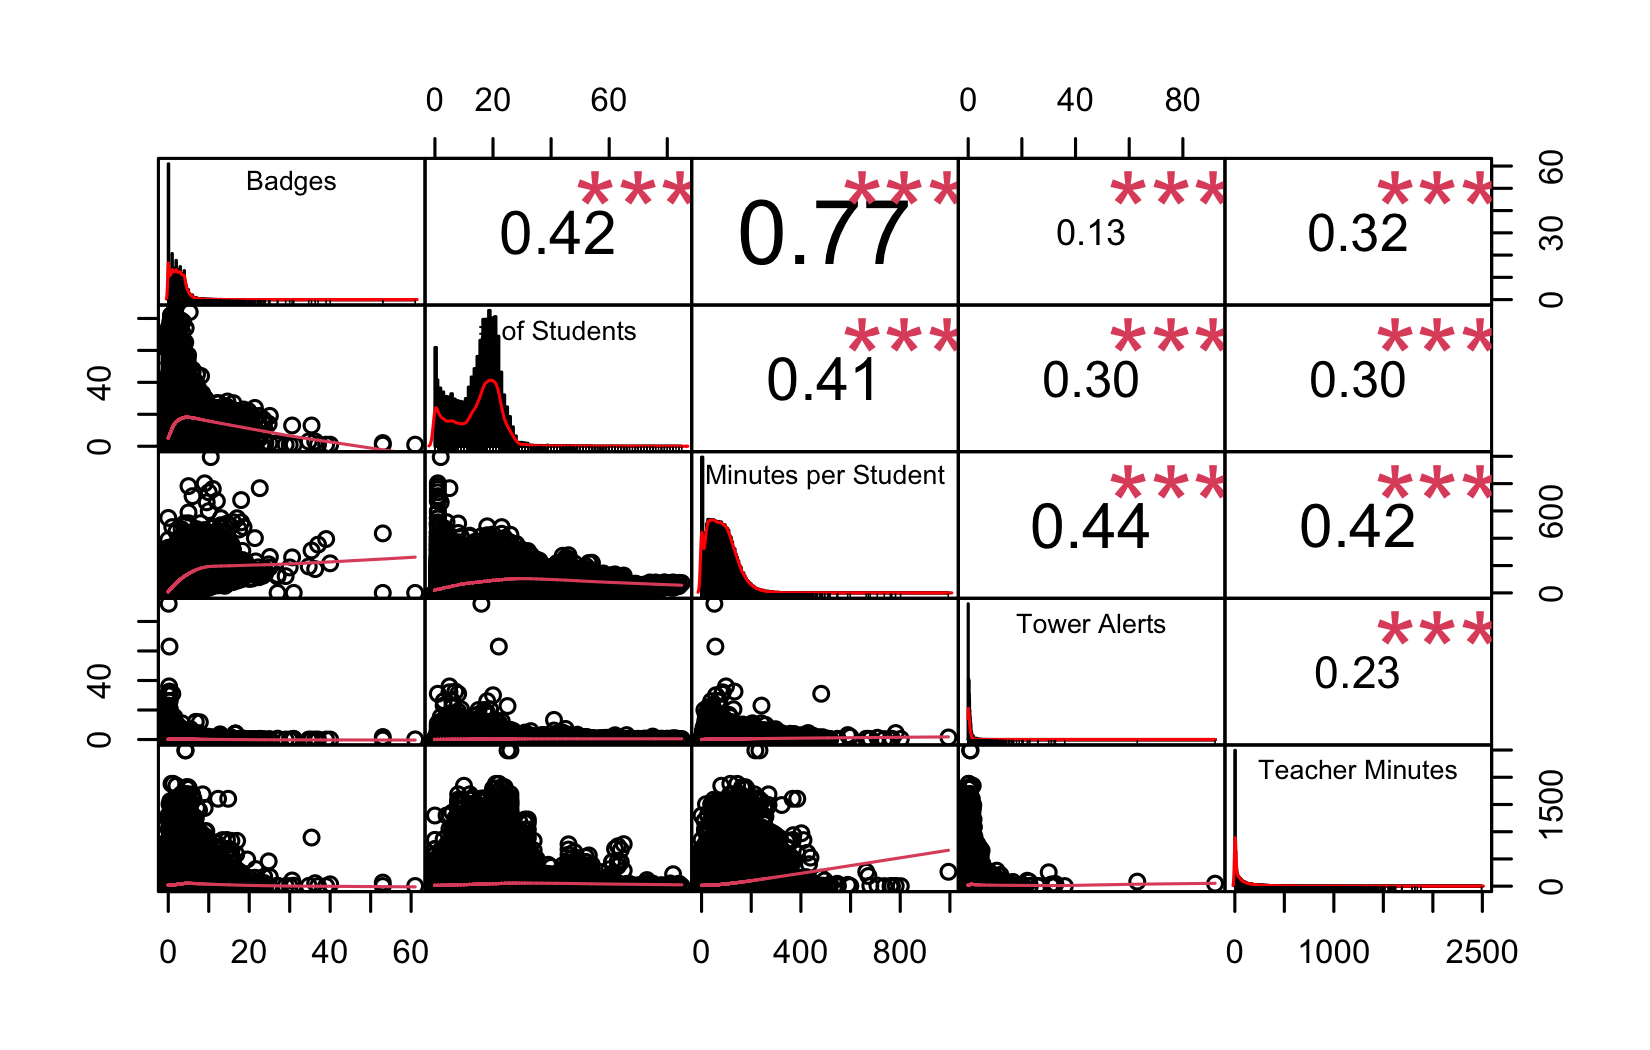
\includegraphics{zearn_files/figure-pdf/fig-corr-1.png}

}

\caption{\label{fig-corr}Correlation coefficients between variables
after stardardization}

\end{figure}%

\subsection{Supplemental Tables}\label{supplemental-tables}

\newpage
\KOMAoptions{paper=landscape,pagesize}
\recalctypearea
{\areaset[current]{\dimexpr\textwidth\relax}{\textheight}
\setlength{\marginparwidth}{0pt}
\scriptsize

\begin{longtable}{l|llllllll}

\caption{\label{tbl-fe-results-statefree}State-Free Panel Logistic
Regression Results}

\tabularnewline

\caption*{
{\large Fixed Effects Logistic Regression Results}
} \\ 
\toprule
\multicolumn{1}{l}{} & \multicolumn{4}{c}{Assessments} & \multicolumn{4}{c}{Pedagogical Knowledge} \\ 
\cmidrule(lr){2-5} \cmidrule(lr){6-9}
\multicolumn{1}{l}{} & \multicolumn{2}{c}{No. Students} & \multicolumn{2}{c}{Struggles} & \multicolumn{2}{c}{Activity} & \multicolumn{2}{c}{No. Students} \\ 
\cmidrule(lr){2-3} \cmidrule(lr){4-5} \cmidrule(lr){6-7} \cmidrule(lr){8-9}
\multicolumn{1}{l}{} & Full & Restricted & Full & Restricted & Full & Restricted & Full & Restricted \\ 
\midrule\addlinespace[2.5pt]
R(t-1) x 
 A(t-1) & -3.192***
(0.961) & — & 0.043
(0.526) & — & -1.188
(0.779) & — & -2.474*
(1.081) & — \\ 
R(t-1) x 
 A(t-2) & 3.742**
(1.225) & 1.287
(0.861) & -1.362*
(0.617) & -0.819
(0.543) & 1.127
(0.819) & 0.106
(0.741) & 3.356*
(1.382) & 0.203
(0.976) \\ 
R(t-2) x 
 A(t-2) & -2.724*
(1.270) & — & 1.358*
(0.652) & — & -1.675*
(0.843) & — & -3.790**
(1.461) & — \\ 
BIC & 71923 & 71920 & 71954 & 71929 & 65463 & 65442 & 65498 & 65489 \\ 
N & 1546 & 1546 & 1546 & 1546 & 1546 & 1546 & 1546 & 1546 \\ 
\bottomrule

\end{longtable}

}
\newpage
\KOMAoptions{paper=portrait,pagesize}
\recalctypearea

\begin{longtable}{l|llll}

\caption{\label{tbl-fe-results}State-Based Panel Logistic Regression
Results}

\tabularnewline

\caption*{
{\large Fixed Effects Logistic Regression Results}
} \\ 
\toprule
\multicolumn{1}{l}{} & \multicolumn{2}{c}{Assessments} & \multicolumn{2}{c}{Pedagogical Knowledge} \\ 
\cmidrule(lr){2-3} \cmidrule(lr){4-5}
\multicolumn{1}{l}{} & \multicolumn{3}{c}{No. Students} & Struggles \\ 
\cmidrule(lr){2-4} \cmidrule(lr){5-5}
\multicolumn{1}{l}{} & Activity & Badges & Activity & Activity \\ 
\midrule\addlinespace[2.5pt]
R(t-1) x 
 A(t-1) & -3.235***
(0.962) & -3.216***
(0.961) & -2.532*
(1.083) & -1.380*
(0.640) \\ 
R(t-1) x 
 A(t-2) & 3.398**
(1.268) & 3.128*
(1.295) & 3.220*
(1.428) & 0.288
(0.618) \\ 
R(t-2) x 
 A(t-2) & -2.714*
(1.270) & -2.743*
(1.269) & -3.809**
(1.461) & -1.622*
(0.678) \\ 
S(t-1) & -1.284*
(0.517) & -1.339*
(0.532) & -2.339***
(0.536) & -2.563***
(0.503) \\ 
S(t-1) x 
 A(t-2) & 0.585
(0.670) & 1.009
(0.728) & 0.022
(0.791) & 0.400
(0.764) \\ 
BIC & 71933 & 71934 & 65472 & 65476 \\ 
N & 1546 & 1546 & 1546 & 1546 \\ 
\bottomrule

\end{longtable}

\subsection{Supplemental Figures}\label{sec-supp-fig}

\begin{figure}

\centering{

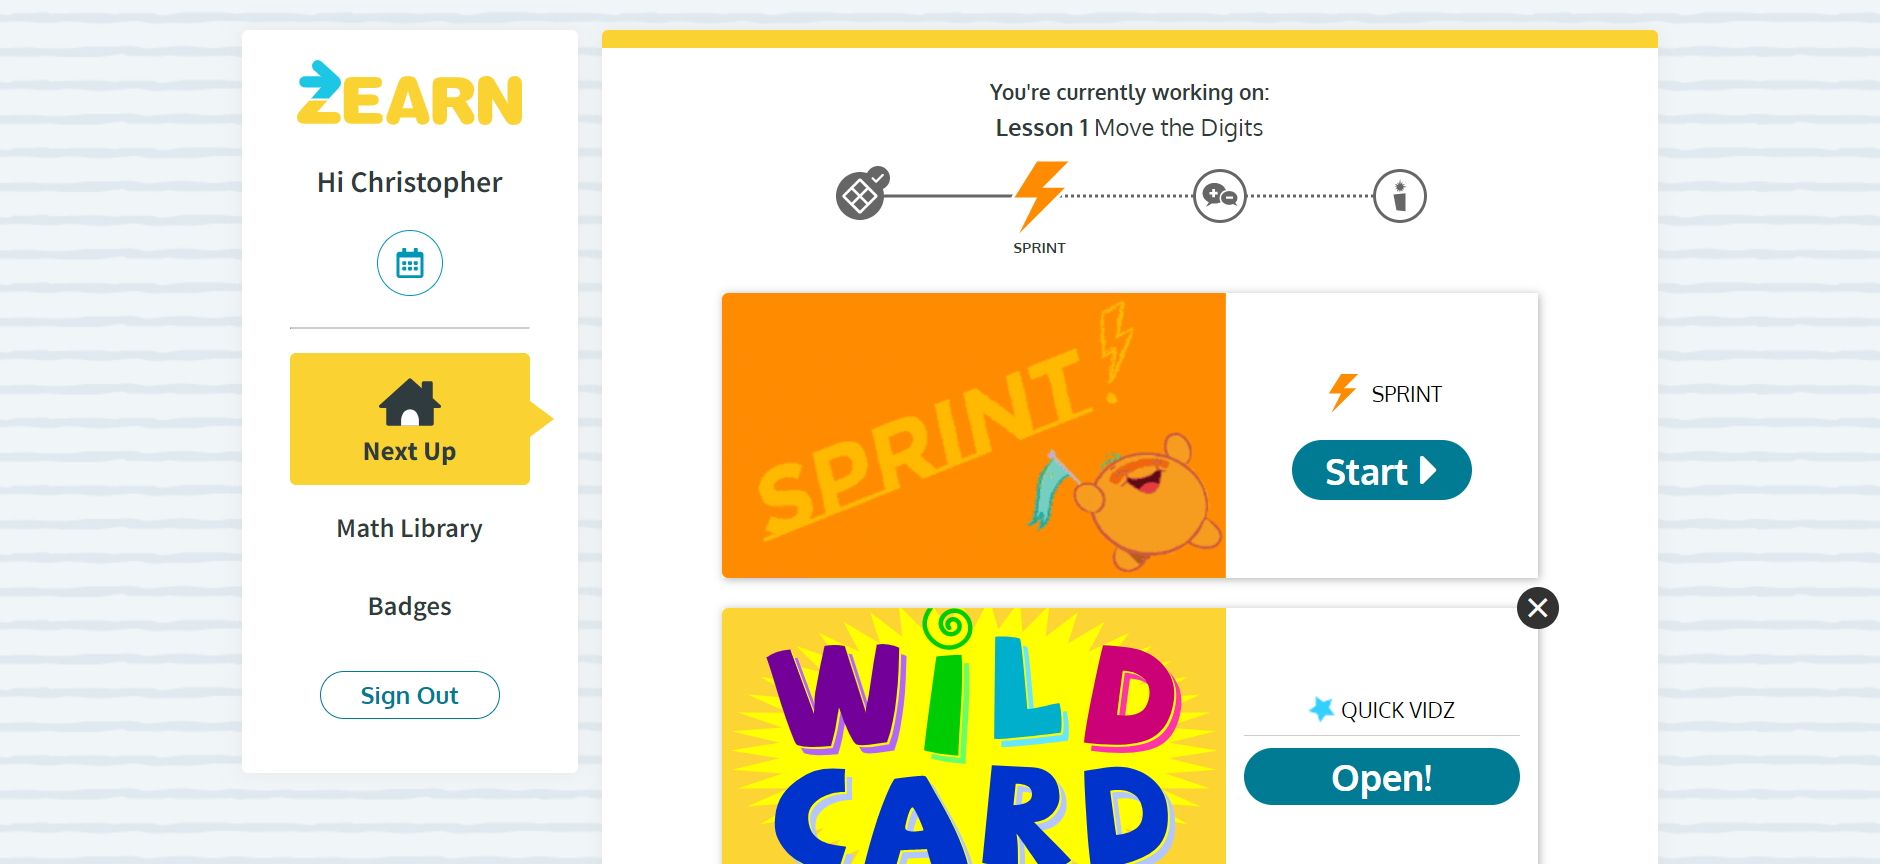
\includegraphics{images/student-feed.PNG}

}

\caption{\label{fig-st-portal}Zearn Student Portal}

\end{figure}%

\begin{figure}

\centering{

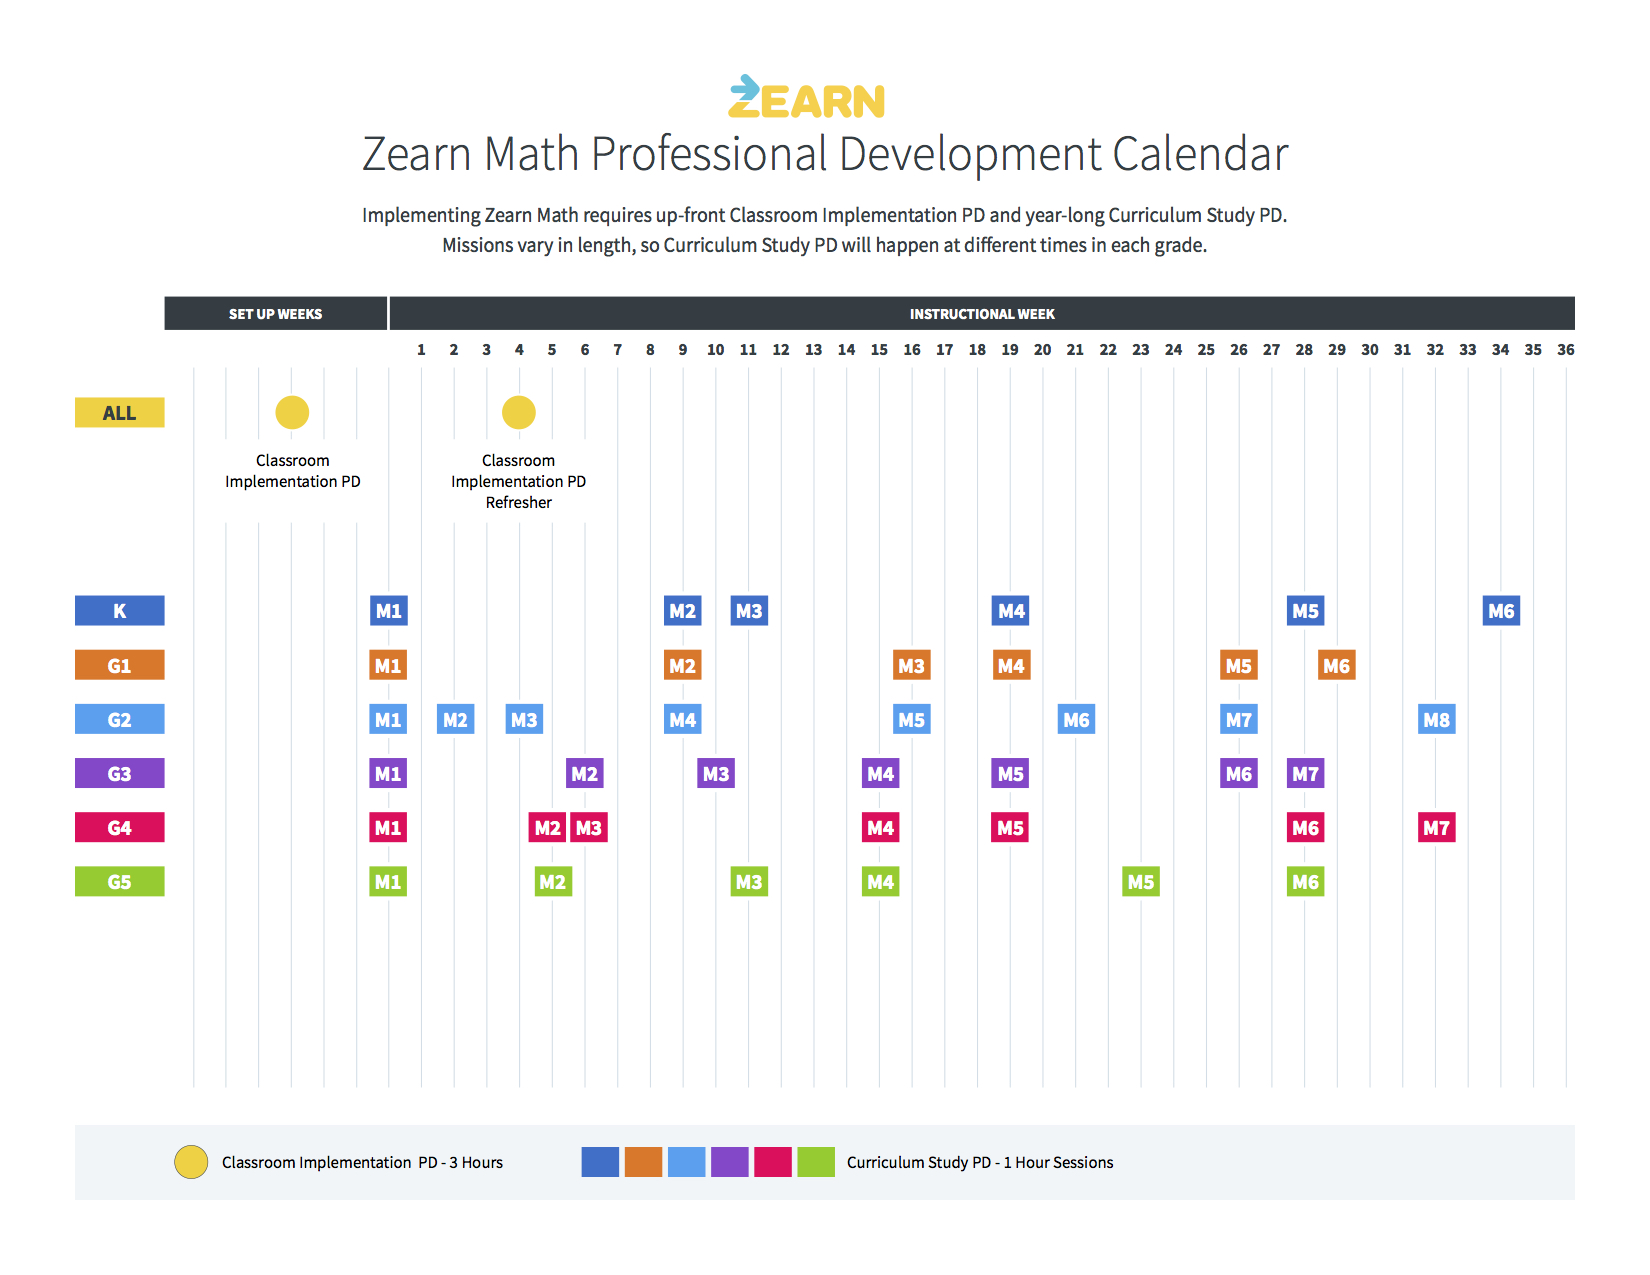
\includegraphics{images/PD-calendar.jpg}

}

\caption{\label{fig-prof-dev}Professional Development Calendar}

\end{figure}%

\newpage{}

\newpage{}




\end{document}
